% Revised manuscript. Analysis items requiring author verification are listed
% separately in submission_notes.md; no numerical results were recalculated.
% v3 (2026-10-29): started from the author's revision; added the description of
% the event content without an added background (Sec. IV A, Sec. V B).
\documentclass[aps,prc,twocolumn,superscriptaddress,nofootinbib,longbibliography,floatfix,10pt]{revtex4-2}
\usepackage{graphicx,amsmath,amssymb,bm,booktabs}
\usepackage[colorlinks=true,linkcolor=blue,citecolor=blue,urlcolor=blue]{hyperref}
\newcommand{\pT}{p_{\mathrm T}}
\newcommand{\vjet}{{v_0^{\mathrm{jet\text{-}UE}}}}
\newcommand{\mpt}{[p_{\mathrm T}]_{\mathrm{ref}}}
\newcommand{\Ctwo}{C_{2,\mathrm{ref}}}
\newcommand{\av}[1]{\left\langle #1\right\rangle}
\newcommand{\Cov}{\operatorname{Cov}}
\newcommand{\Var}{\operatorname{Var}}
\newcommand{\dd}{\mathrm d}
% allow two page-wide figures per float page (appendix figures)
\renewcommand{\dbltopfraction}{0.95}
\renewcommand{\dblfloatpagefraction}{0.8}
\setcounter{dbltopnumber}{3}
\begin{document}
\title{Probing jet-induced medium response with jet--underlying-event transverse-momentum correlations}
\author{Somadutta Bhatta}
\affiliation{Institute for Gravitational and Subatomic Physics (GRASP), Utrecht University, Utrecht, The Netherlands}
\affiliation{Nikhef, National Institute for Subatomic and High Energy Physics, Amsterdam, The Netherlands}
\author{Preeti Dhanker}
\affiliation{Institute for Gravitational and Subatomic Physics (GRASP), Utrecht University, Utrecht, The Netherlands}
\affiliation{Nikhef, National Institute for Subatomic and High Energy Physics, Amsterdam, The Netherlands}
\date{\today}
\author{Marco Van Leeuwen}
\affiliation{Institute for Gravitational and Subatomic Physics (GRASP), Utrecht University, Utrecht, The Netherlands}
\affiliation{Nikhef, National Institute for Subatomic and High Energy Physics, Amsterdam, The Netherlands}
\begin{abstract}
The energy deposited by a quenched jet modifies both its internal structure and the surrounding particle production. Correlating these two regions provides a way to study medium response beyond the modification of an average jet spectrum. We propose $\vjet(\pT)$, which correlates event-by-event changes of the normalized in-cone charged-particle spectrum with the mean transverse momentum of reference particles outside the cone. We derive its leading relation to a connected two-particle density and establish how its particle-number and centered-momentum weights differ from the energy weights of energy--energy correlators. Using JEWEL for O+O collisions at $\sqrt{s_{\mathrm{NN}}}=5.36$~TeV, we find no resolved modification in the calculation without recoils, whereas retaining recoils produces a positive change for probes with $1<\pT<6$~GeV/$c$ and a predominantly negative change for $12<\pT<100$~GeV/$c$. The soft-probe change grows between $R=0.1$ and $0.4$ and remains comparable at $R=0.8$. Embedding in an independent thermal background demonstrates the importance of the reference-fluctuation normalization and quantifies residual background-induced changes using JEWEL vacuum and PYTHIA baselines. For the specified simulated samples and uncertainty prescription, the soft-probe sensitivity reaches $Z=5.4$ at $R=0.8$ for $40$--$60$~GeV/$c$ jets. The same qualitative separation is obtained with perpendicular-cone and constituent subtraction. These results motivate jet--UE spectral correlations as a complementary probe of medium response; establishing collective thermalization requires calculations with a dynamically evolving bulk medium.
\end{abstract}
\maketitle

\section{Introduction}\label{sec:intro}
Energetic quarks and gluons lose energy as they propagate through the quark--gluon plasma (QGP). The accompanying redistribution of energy and momentum modifies the parton shower and excites the surrounding medium. Measurements of jet structure therefore contain contributions from the modified shower, particles associated with the medium response, and the underlying event (UE). A central challenge is to identify observables that distinguish these contributions through their correlations, rather than through the soft-particle yield alone.

Recent measurements provide direct motivation for studying the particles surrounding a hard probe. Correlations of Z bosons with charged hadrons show modifications consistent with medium response, and dijet--hadron correlations provide evidence for a diffusion wake~\cite{CMSZ,CMSWake}. Energy--energy correlators (EECs) reveal modifications of the angular distribution of momentum inside jets in Pb--Pb collisions~\cite{CMSEEC}. Their interpretation involves both changes of the shower and the response of the medium. The observation of suppressed charged-particle production in O+O collisions~\cite{CMSOO} extends this question to a smaller collision system, where the UE is lower than in central Pb--Pb collisions.

A complementary approach is provided by event-by-event transverse-momentum fluctuations. In the bulk, the differential observable $v_0(\pT)$ measures how the particle spectrum changes with the event mean transverse momentum~\cite{Schenke,ATLASv0,ALICEv0}. The normalized spectrum distinguishes a change of shape from a common rescaling of the yield. Its normalization and event-activity definition must nevertheless be specified: the zero crossing is not, by itself, a unique dynamical scale~\cite{BhattaShape}. These considerations suggest extending the spectral-fluctuation method to two physically distinct regions, a jet cone and the surrounding event.

In this work we introduce $\vjet(\pT)$ to ask whether a change in the fraction of particles at a given momentum inside a jet accompanies a change in the mean momentum outside it. A correlation can already arise in vacuum from fragmentation, recoil activity, conservation laws, and event selection. The physics information is therefore in its modification relative to a controlled baseline. Medium response can change this correlation by redistributing particles on both sides of the cone boundary. The observable is inspired by bulk radial-flow measurements, but its definition does not assume that the measured correlation is collective.

The contribution of this study has two parts. We first identify the pair weights and normalization that make the observable sensitive to spectral redistribution, and clarify its relation to EECs. We then compare JEWEL calculations with and without retained recoils, together with vacuum samples embedded in the same independent background. This separates the response-sensitive modification within the model from the change induced by the background level alone. The main finding is that the recoil-retaining calculation modifies the soft and hard probe correlations in opposite directions, while the calculation without recoils remains compatible with the vacuum baseline at the available precision. We examine this separation versus jet radius, reference selection, and subtraction method, and distinguish the change of the signal amplitude from the change of its statistical sensitivity.

\section{Observable and physical interpretation}\label{sec:observable}
\subsection{Correlating spectral shape with the reference mean}
For each selected leading jet, let $n_b$ be the charged-particle count in a probe momentum bin $b$ and let $N$ be the count summed over the probe normalization range. Define
\begin{equation}
 f_b=\frac{n_b}{N},\qquad N=\sum_b n_b,\qquad \sum_b f_b=1.
 \label{eq:f}
\end{equation}
The notation $f(\pT)$ denotes the same binned fraction when displaying its momentum dependence. The momentum bins entering $N$ must coincide with those entering the sum. Multiplying every $n_b$ by a common factor leaves $f_b$ unchanged. By contrast, moving particles from one bin to another changes the corresponding fractions. Thus $f_b$ describes the shape of the spectrum independently of a pure rescaling of its normalization.

The reference consists of charged particles with $0.2<\pT<3$~GeV/$c$ outside the jet cone and the two perpendicular cones defined in Sec.~\ref{sec:setup}. Its scalar transverse-momentum sum $P_{\mathrm{ref}}$, multiplicity $M$, and event mean are
\begin{equation}
 P_{\mathrm{ref}}=\sum_{j\in\mathrm{ref}}p_{\mathrm T,j},\qquad
 M=N_{\mathrm{ref}},\qquad \mpt=\frac{P_{\mathrm{ref}}}{M}.
 \label{eq:ref}
\end{equation}
The mean distinguishes a harder reference spectrum from a larger number of reference particles with the same spectrum.

Within a fixed event class, $\av X$ denotes the event average with the generator weights and $\delta X=X-\av X$. The observable is
\begin{equation}
 \vjet(b)=\frac{\Cov(f_b,\mpt)}{\av{f_b}\sqrt{\Ctwo}},
 \qquad \Cov(X,Y)=\av{\delta X\delta Y}.
 \label{eq:v0}
\end{equation}
A positive value means that the fraction in bin $b$ tends to increase in events with a larger reference mean momentum; a negative value means that it tends to decrease. Dividing by $\av{f_b}$ expresses the covariance relative to the mean bin population. The reference scale is the distinct-particle correlator
\begin{equation}
 \Ctwo=\av{\frac{\sum_{i\ne j\in\mathrm{ref}}
 (p_{\mathrm T,i}-\mu)(p_{\mathrm T,j}-\mu)}{M(M-1)}}.
 \label{eq:c2}
\end{equation}
Here $\mu=\av{\mpt}$. Equation~\eqref{eq:c2} specifies an average of the per-event ordered-pair correlator~\cite{BhattaCumulants}; replacing it by a ratio of ensemble pair sums would change the event weighting. Self-pairs are excluded, so $\Ctwo$ is not generally equal to $\Var(\mpt)$. Its square root has momentum units and makes Eq.~\eqref{eq:v0} dimensionless. The estimator requires $N>0$, $M\ge2$, $\Ctwo>0$, and a nonzero $\av{f_b}$. It is a reference-normalized covariance, not a Pearson coefficient bounded by unity.

The normalization of the probe gives the exact constraint
\begin{equation}
 \sum_b\Cov(f_b,\mpt)=0,\qquad
 \sum_b\av{f_b}\vjet(b)=0.
 \label{eq:sumrule}
\end{equation}
For positive mean fractions, a nonzero correlation must contain compensating positive and negative contributions. The constraint does not determine their ordering in momentum, the number of crossings, or a crossing momentum. It expresses conservation of the normalized particle fraction, not conservation of the jet energy. These identities apply within a common event class and acceptance; combining separately normalized classes requires retaining their weights explicitly.

\subsection{Why the pair weights select changes of shape}
The connection to two-particle correlations follows by expanding the two fluctuating denominators. Define the ratios of means
\begin{equation}
 \bar f_b=\frac{\av{n_b}}{\av N},\qquad
 \bar p_{\mathrm{ref}}=\frac{\av{P_{\mathrm{ref}}}}{\av M}.
 \label{eq:means}
\end{equation}
These differ in general from $\av{f_b}$ and $\mu$, respectively. To first order in fluctuations of the extensive quantities,
\begin{align}
 \delta f_b&\simeq\frac{\delta n_b-\bar f_b\delta N}{\av N},\label{eq:expandf}\\
 \delta\mpt&\simeq\frac{\delta P_{\mathrm{ref}}-\bar p_{\mathrm{ref}}\delta M}{\av M}.
 \label{eq:expandref}
\end{align}
The first subtraction removes the bin population expected from a change of the total count at fixed spectral shape. For example, a bin containing one fifth of the particles gains two particles when the total increases by ten at unchanged shape. The second subtraction removes the reference momentum expected from the additional reference particles at unchanged mean momentum. The remaining fluctuations therefore measure spectral redistribution and a change of reference mean, respectively.

Multiplying Eqs.~\eqref{eq:expandf} and \eqref{eq:expandref} gives the leading covariance,
\begin{align}
 \Cov(f_b,\mpt)\simeq{}&\frac{1}{\av N\av M}\Big[\Cov(n_b,P_{\mathrm{ref}})\nonumber\\
 &-\bar p_{\mathrm{ref}}\Cov(n_b,M)
 -\bar f_b\Cov(N,P_{\mathrm{ref}})\nonumber\\
 &+\bar f_b\bar p_{\mathrm{ref}}\Cov(N,M)\Big].
 \label{eq:fourterms}
\end{align}
This is second order in fluctuations, obtained from first-order expansions of the two ratios. It is not an exact replacement for Eq.~\eqref{eq:v0} when denominator fluctuations are large.

Let $\chi_b(i)$ equal one when particle $i$ lies in bin $b$ and zero otherwise. The two centered additive sums are
\begin{align}
 \Delta n_b&=n_b-\bar f_bN=\sum_{i\in\mathrm{cone}}[\chi_b(i)-\bar f_b],\nonumber\\
 \Delta P_{\mathrm{ref}}&=P_{\mathrm{ref}}-\bar p_{\mathrm{ref}}M
 =\sum_{j\in\mathrm{ref}}[p_{\mathrm T,j}-\bar p_{\mathrm{ref}}].
 \label{eq:residuals}
\end{align}
Both have zero ensemble mean. Consequently,
\begin{align}
 \Cov(f_b,\mpt)&\simeq\frac{\av{\sum_{i\in\mathrm{cone}}\sum_{j\in\mathrm{ref}}w_b(i)w_{\mathrm{ref}}(j)}}{\av N\av M},\nonumber\\
 w_b(i)&=\chi_b(i)-\bar f_b,\nonumber\\
 w_{\mathrm{ref}}(j)&=p_{\mathrm T,j}-\bar p_{\mathrm{ref}}.
 \label{eq:pairs}
\end{align}
The cone weight is $1-\bar f_b$ inside the selected bin and $-\bar f_b$ outside it. The reference weight is positive above its centering momentum and negative below. These forms follow from the ratio expansions; they remove the two particle-number contributions in Eq.~\eqref{eq:fourterms}. A pair's contribution depends on the product of both weights. Its sign cannot be inferred from the reference particle's momentum alone. The disconnected contribution, the product of the separate mean sums, vanishes. Disjoint regions eliminate same-particle pairs but do not eliminate correlations from fragmentation, recoil jets, or conservation laws.

\section{Relation to energy--energy correlators}\label{sec:eec}
Write $x=(\pT,\eta,\varphi)$, with $\dd x=\dd\pT\dd\eta\dd\varphi$. In coordinates relative to the selected jet, define the mean single-particle density $\rho_1$, the ordered distinct-pair density $\rho_2$, and their connected part,
\begin{align}
 \rho_1(x)&=\av{\sum_i\delta(x-x_i)},\nonumber\\
 \rho_2(x_1,x_2)&=\av{\sum_{i\ne j}\delta(x_1-x_i)\delta(x_2-x_j)},\nonumber\\
 C(x_1,x_2)&=\rho_2(x_1,x_2)-\rho_1(x_1)\rho_1(x_2).
 \label{eq:density}
\end{align}
A density integrated over a coordinate cell gives the corresponding mean count. The subtraction removes the pair contribution obtained by independently combining the one-particle distributions from the same selected ensemble. For the two disjoint regions, Eq.~\eqref{eq:pairs} becomes
\begin{multline}
 \Cov(f_b,\mpt)\simeq\frac{1}{\av N\av M}
 \int_{\mathrm{cone}}\dd x_1\int_{\mathrm{ref}}\dd x_2\\
 \times[\chi_b(x_1)-\bar f_b]
 [p_{\mathrm T,2}-\bar p_{\mathrm{ref}}]C(x_1,x_2).
 \label{eq:corr}
\end{multline}
The reference mask includes the momentum acceptance and perpendicular-cone exclusions. It cannot be replaced by a radial cut alone.

For comparison, define a connected cross-region energy correlator with a fixed momentum normalization $p_{\mathrm T,*}^{\mathrm{jet}}$,
\begin{multline}
 {\cal E}^{\mathrm{conn}}_{\mathrm{jet,ref}}(\theta)
 =\frac{1}{(p_{\mathrm T,*}^{\mathrm{jet}})^2}
 \int_{\mathrm{cone}}\dd x_1\int_{\mathrm{ref}}\dd x_2\\
 \times p_{\mathrm T,1}p_{\mathrm T,2}
 \delta(\theta-\theta_2)C(x_1,x_2),
 \label{eq:eec}
\end{multline}
where $\theta_2=\sqrt{(\eta_2-\eta_{\mathrm{jet}})^2+(\Delta\varphi_{2,\mathrm{jet}})^2}$ is the reference particle's distance from the jet axis. The Dirac delta assigns the pair to its reference-angle bin. This explicitly connected, axis-angle observable is a comparison construction. The conventional in-jet EEC instead resolves the separation between two in-jet particles and is ordinarily defined using the full pair density, without this connected subtraction~\cite{Basham,Andres}. A particle outside the cone can be arbitrarily close to a particle inside it: $\theta_2>R$ does not imply a pair separation greater than $R$.

Integrating Eq.~\eqref{eq:eec} over the full selected reference angle gives
\begin{equation}
 \int\dd\theta\,{\cal E}^{\mathrm{conn}}_{\mathrm{jet,ref}}
 =\frac{\Cov(P_{\mathrm{cone}},P_{\mathrm{ref}})}{(p_{\mathrm T,*}^{\mathrm{jet}})^2},
 \label{eq:inteec}
\end{equation}
where $P_{\mathrm{cone}}=\sum_{i\in\mathrm{cone}}p_{\mathrm T,i}$ is a scalar sum, not the reconstructed vector jet momentum. If an event-dependent jet momentum is used in the denominator, that factor must remain inside the event average. A finite jet-momentum bin does not make these definitions exactly equivalent.

Equations~\eqref{eq:corr} and \eqref{eq:eec} expose the complementarity. The energy correlator weights a pair by its momentum product and retains angular structure. The leading $\vjet$ numerator retains separate probe bins, subtracts the change proportional to the mean cone spectrum, and correlates the remaining shape change with centered reference momentum. A change of soft-particle abundance can contribute without an additional factor of the probe momentum. The full $\vjet$ also requires the mean fraction and a reference--reference correlator; it is not a linear functional of $C$ and cannot be reconstructed from an angular EEC alone.

The advantage is therefore a particular sensitivity to spectral redistribution and its relation to the surrounding mean momentum, rather than a general superiority to EECs. A connected energy correlator can also be negative. Neither a signed reference weight nor a sign change establishes a thermalized response. Particle-count fractions additionally depend on thresholds and collinear splitting and do not inherit the infrared-and-collinear safety of an ideal inclusive energy correlator.

Varying $R$ tests the stability and geometrical dependence of the measurement, but does not directly recover an angular distribution. It changes the probe particles, reference exclusions, average weights, reference normalization, and potentially the jet axis and selected event population. An annular measurement would instead hold the jet selection and probe fixed while varying only a specified reference domain. This distinction is especially relevant here because the tracking acceptance changes for $R=0.8$.

\section{Simulation and analysis}\label{sec:setup}
\subsection{Generator configurations and embedded background}
We use JEWEL~2.4.0~\cite{ZappFramework,ZappManual} for pp and O+O collisions at $\sqrt{s_{\mathrm{NN}}}=5.36$~TeV, with CT18ANLO~\cite{CT18} and EPPS21~\cite{EPPS21} parton distributions. The O+O calculation uses the longitudinally expanding Bjorken medium implemented in JEWEL, with initialization time $\tau_i=0.4$~fm/$c$ and temperature $T_i=0.43$~GeV. The temperature is obtained in the analysis by scaling the default Pb--Pb value of $0.59$~GeV using the O+O multiplicity. The generated O+O sample is minimum bias, corresponding to 0--100\% centrality.

Three configurations are compared: vacuum, a medium calculation without retained recoils, and a medium calculation with retained recoils. The second contains medium modifications of the hard shower but omits the final-state recoil contribution. The third also retains the struck scattering centers as the model's representation of medium response. Their pre-scattering thermal momenta are removed by event-level constituent subtraction~\cite{Milhano}, with a maximum matching distance $\Delta R_{\max}=1.0$ for the nominal result and $0.5$ for a variation. This thermal-momentum subtraction is distinct from subtracting the independently embedded UE below. JEWEL recoils do not constitute a hydrodynamic wake and do not demonstrate equilibration with an expanding bulk medium.

Vacuum baselines are supplied by JEWEL and PYTHIA~8.317~\cite{Pythia}, the latter using the Monash tune~\cite{Monash} with multiparton interactions (MPI) either enabled or disabled. Samples use a hard-scattering generation bias proportional to $\hat p_{\mathrm T}^{4.5}$ above $\hat p_{\mathrm T}=5$~GeV/$c$, together with compensating event weights. Each sample contains $10^7$ generated events except PYTHIA without MPI, which contains $2\times10^6$.

Without an added background, a JEWEL event contains only particles from the hard scattering. These are the selected jet, the recoiling jet and other wide-angle radiation, and, in the recoil-retaining calculation, the hadronized recoil partons. The JEWEL medium is a temperature profile from which the shower partons scatter; it does not itself produce particles. The reference region is therefore populated by activity of the same hard event, not by a bulk UE. The interaction with the medium enters the observable in two ways. Energy loss modifies the in-cone spectrum, which is tested by the calculation without recoils. Retained recoils add correlated particles both inside the cone and in the reference region, which is tested by the recoil-retaining calculation. The result without an added background thus isolates the sensitivity of $\vjet$ to these two mechanisms in an idealized limit in which nothing else contributes to the reference. It is not a measurable configuration. The embedded-background samples described next test how much of this sensitivity remains when the reference also contains particles unrelated to the jet.

The JEWEL setup does not generate the complete final-state bulk event. We therefore superimpose an independent background of charged pions, with mean transverse momentum $0.7$~GeV/$c$ and charged-particle pseudorapidity density $\dd N_{\mathrm{ch}}/\dd\eta=42$ or $135$. These densities approximate the measured minimum-bias and 0--5\% O+O values~\cite{CMSMultiplicity}. The larger density is an embedding variation, not a new central O+O medium calculation. The same background prescription is applied to the vacuum baselines. This construction tests the consequences of extra particles and their subtraction; it does not include collective bulk correlations or a dynamical interaction between the added particles and the jet.

\subsection{Jet selection, probes, and reference regions}
Charged particles with $\pT>0.15$~GeV/$c$ are clustered with anti-$k_t$~\cite{AntiKt,FastJet}. The tracking acceptance is $|\eta|<0.9$ for $R=0.1$, $0.2$, and $0.4$, and $|\eta|<2.5$ for $R=0.8$. The jet axis satisfies $|\eta_{\mathrm{jet}}|<\eta_{\max}-R$. Two cones centered at the jet pseudorapidity and at azimuths $\varphi_{\mathrm{jet}}\pm\pi/2$ estimate the background momentum density $\rho$ and the background yield $b_b$ expected in each probe bin. Jet classes are selected using
\begin{equation}
 p_{\mathrm T}^{\mathrm{jet,corr}}=p_{\mathrm T}^{\mathrm{jet}}-\rho A,
 \label{eq:jetcorr}
\end{equation}
where $A$ is the jet area. The two main classes are $20$--$40$ and $40$--$60$~GeV/$c$.

We compare the raw fraction $f_b$, the normalized perpendicular-cone-subtracted spectrum, and the spectrum after constituent subtraction~\cite{Berta}. Writing $B=\sum_b b_b$ and $N_{\mathrm{cs}}=\sum_b n_{b,\mathrm{cs}}$, their definitions are
\begin{equation}
 f_{b,\mathrm{sub}}=\frac{n_b-b_b}{N-B},\qquad
 f_{b,\mathrm{cs}}=\frac{n_{b,\mathrm{cs}}}{N_{\mathrm{cs}}}.
 \label{eq:subtracted}
\end{equation}
All fractions use the same stated probe normalization range. The subtraction can yield signed bin contents; $f_{b,\mathrm{sub}}$ is then a normalized subtracted spectrum rather than a probability. Only events with a valid nonzero normalization can enter its estimator. The nominal reference excludes the jet and perpendicular cones. A second selection uses reference particles separated by $|\eta-\eta_{\mathrm{jet}}|>R+0.5$.

The derivation in Sec.~\ref{sec:observable} applies directly to raw particle counts. For $f_{b,\mathrm{sub}}$, the same algebra uses $n_b-b_b$ and $N-B$, introducing covariances involving the background estimator. Constituent subtraction also modifies the particle sample and its selection. Thus the subtraction comparison is a test of the full estimator, not a consequence of the raw cone--reference identity alone.

\subsection{Event classes and statistical treatment}
The moments are accumulated in narrow midrapidity multiplicity classes, with the generator event weights included. The normalized result is evaluated within each class and combined using its event weight. If $a$ labels a multiplicity class and $W_a$ its fraction of the total event weight, this prescription is
\begin{equation}
 \vjet_{\mathrm{combined}}(b)=\sum_a W_a\vjet_a(b),\qquad \sum_a W_a=1.
 \label{eq:classes}
\end{equation}
It differs in general from forming a ratio after pooling the moments over a broad class. Class-specific centers and the reference correlator must be used consistently.

Uncertainties are estimated with 40 Poisson bootstrap replicas. Probe-bin edges are $0.2$, $0.5$, $1$, $2$, $3$, $6$, $12$, $30$, and $100$~GeV/$c$. For merging adjacent bins within a class, the covariances and mean fractions are summed before evaluating Eq.~\eqref{eq:v0}. This produces the estimator for the merged bin. The soft- and hard-range summaries below instead use inverse-variance-weighted averages of the differential results over $1<\pT<6$ and $12<\pT<100$~GeV/$c$, respectively. These summaries are not identical to a single merged-bin estimator.

\subsection{Medium modification and the background baseline}
At fixed embedded background level $U$, define the model medium modification
\begin{equation}
 S(b;U)=\vjet_{\mathrm{medium}+U}(b)-\vjet_{\mathrm{vacuum}+U}(b).
 \label{eq:signal}
\end{equation}
It is evaluated separately with and without retained recoils. For a vacuum generator $g$, the background-induced change is
\begin{equation}
 F_g(b;U)=\vjet_{g+U}(b)-\vjet_g(b),\quad
 \bar F=\tfrac12(F_{\mathrm J}+F_{\mathrm P}),
 \label{eq:background}
\end{equation}
where J and P denote JEWEL vacuum and PYTHIA. The baseline includes changes from embedding, reconstruction, selection, and normalization. Independent added particles need not leave the final selected observable unchanged.

An experimental O+O--pp difference would require a background correction and a test of any remaining vacuum-baseline differences. Within one generator, the identity
\begin{equation}
 \vjet_{\mathrm{medium}+U}-\vjet_{\mathrm{vacuum}}
 =S+F_{\mathrm J}
 \label{eq:decomposition}
\end{equation}
shows that $S$ already compares samples at the same background level. Subtracting $F$ again from $S$ would double-count the correction.

To compare the simulated separation with the estimated uncertainty of such a background correction, we retain the diagnostic used in the analysis,
\begin{equation}
 Z=\frac{S}{\sqrt{\sigma_S^2+\sigma_{\bar F}^2+\delta_F^2}},\qquad
 \delta_F=\frac{|F_{\mathrm J}-F_{\mathrm P}|}{2}.
 \label{eq:Z}
\end{equation}
Here $\sigma_S$ is the statistical uncertainty of the medium difference, $\sigma_{\bar F}$ is the statistical uncertainty assigned to the mean background correction, and $\delta_F$ estimates the spread of the two baselines. Equation~\eqref{eq:Z} treats these contributions in quadrature. It is a signed sensitivity diagnostic for the generated samples and this uncertainty prescription, not a projected significance for a specified experimental luminosity or a hypothesis-test probability. Shared samples and correlations across probe bins, subtraction methods, and radii require a joint covariance treatment for a combined inference.

\section{Results}\label{sec:results}
\subsection{Vacuum correlations and the role of MPI}
\begin{figure*}[t]
 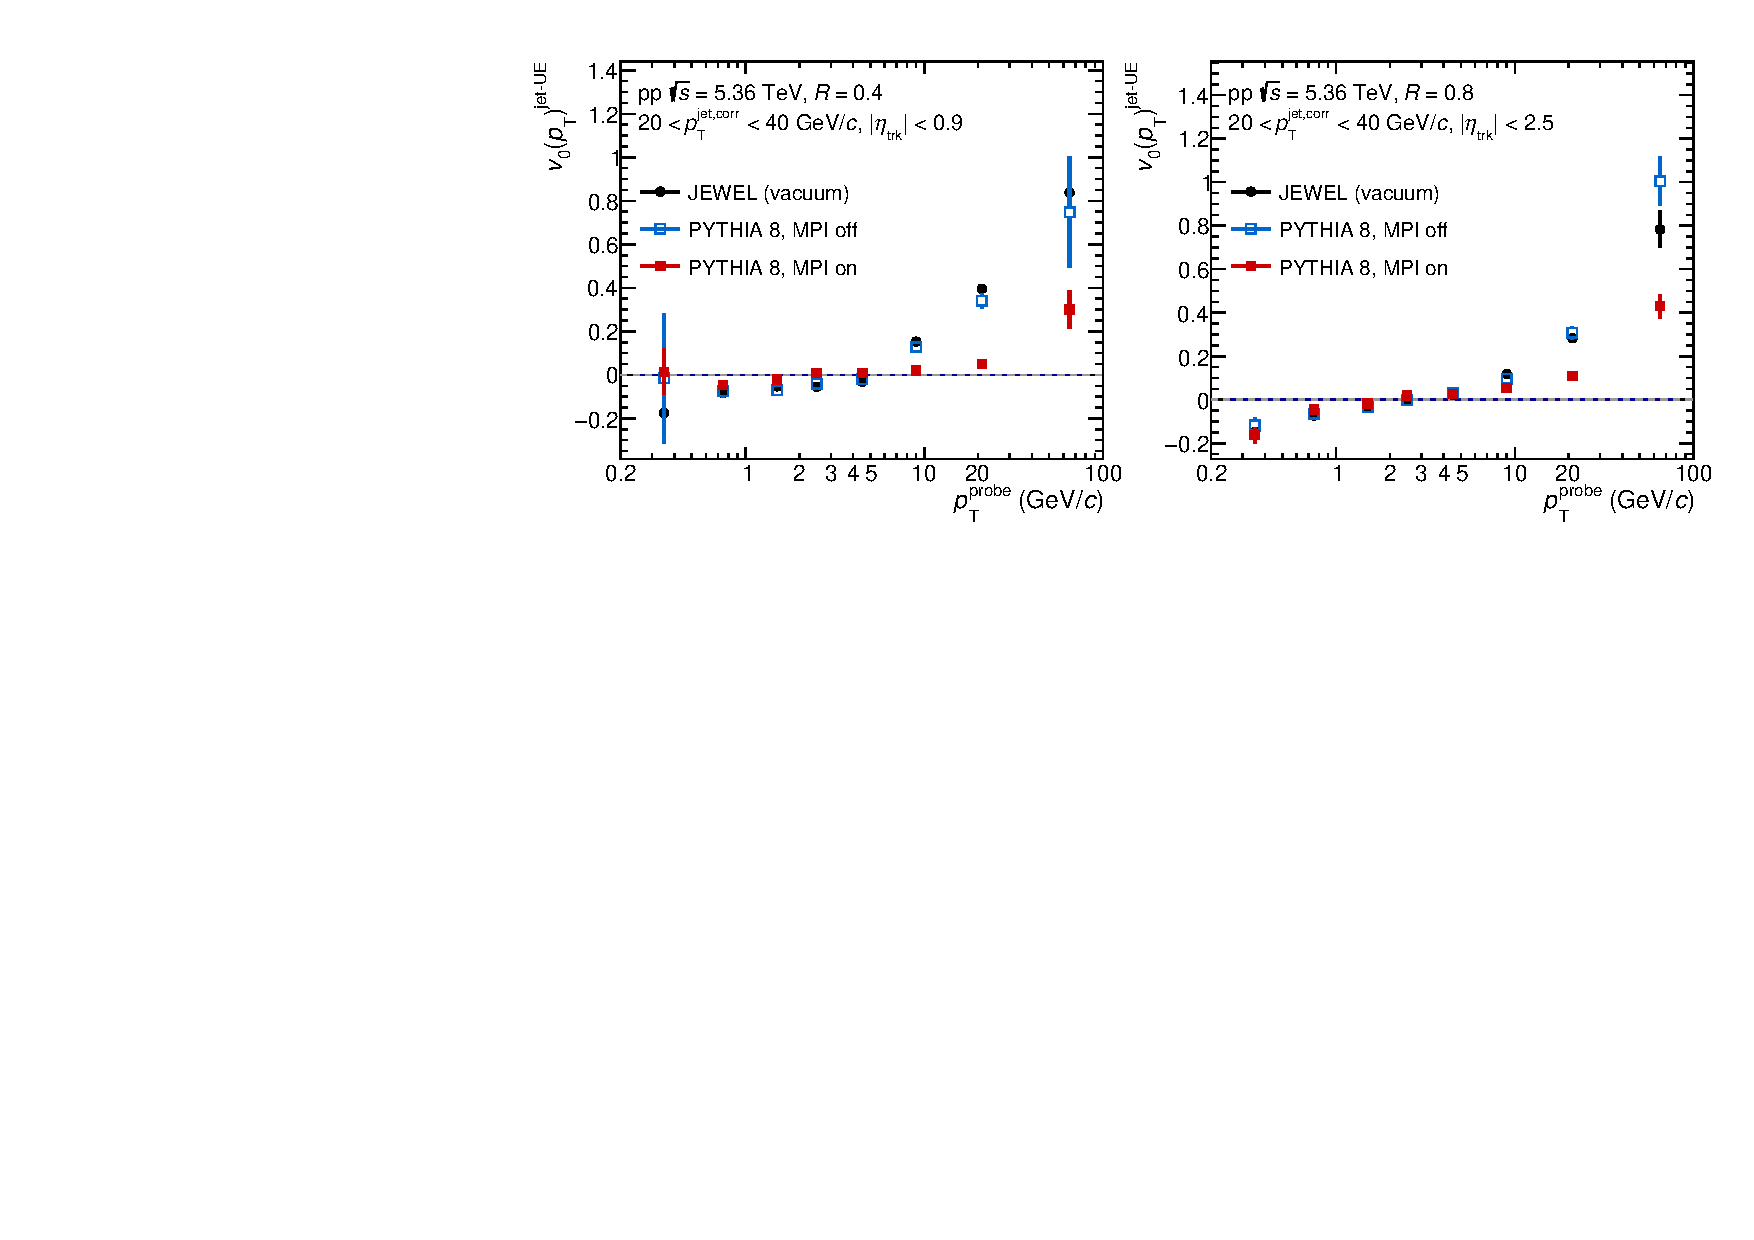
\includegraphics[width=0.98\textwidth]{figs/fig_pp.pdf}
 \caption{$\vjet(\pT)$ in pp collisions for $20<p_{\mathrm T}^{\mathrm{jet,corr}}<40$~GeV/$c$, using the perpendicular-cone-subtracted probe. Left: $R=0.4$ with $|\eta_{\mathrm{trk}}|<0.9$. Right: $R=0.8$ with $|\eta_{\mathrm{trk}}|<2.5$. JEWEL vacuum is compared with PYTHIA~8 with MPI disabled and enabled. Error bars represent bootstrap statistical uncertainties.}
 \label{fig:pp}
\end{figure*}
Figure~\ref{fig:pp} establishes that a sizable jet--reference correlation exists without a medium. The vacuum curves are negative at low probe momentum and positive at high momentum, with a crossing near $3$--$6$~GeV/$c$. This pattern means that events with a larger reference mean tend to have a smaller soft fraction and a larger hard fraction in the selected jet. The compensation is consistent with Eq.~\eqref{eq:sumrule}; the particular momentum ordering and crossing position are properties of these samples, not predictions of that constraint.

JEWEL vacuum and PYTHIA without MPI give compatible high-momentum results. At $R=0.4$ and $12<\pT<30$~GeV/$c$, their values are $0.40\pm0.02$ and $0.34\pm0.04$, respectively. Enabling MPI in PYTHIA reduces the result to $0.05\pm0.02$. This establishes a substantial sensitivity to the vacuum event environment. It should not be interpreted as a pure dilution test: MPI can change the reference composition, correlations, and leading-jet selection, and is not equivalent to adding independent particles after event generation. JEWEL vacuum O+O and pp results, $0.38\pm0.02$ and $0.40\pm0.02$ in this bin, show no resolved baseline difference at the present precision. This check does not establish the absence of nuclear parton-distribution effects in other selections.

\subsection{Separation of the calculations with and without recoils}
\begin{figure*}[t]
 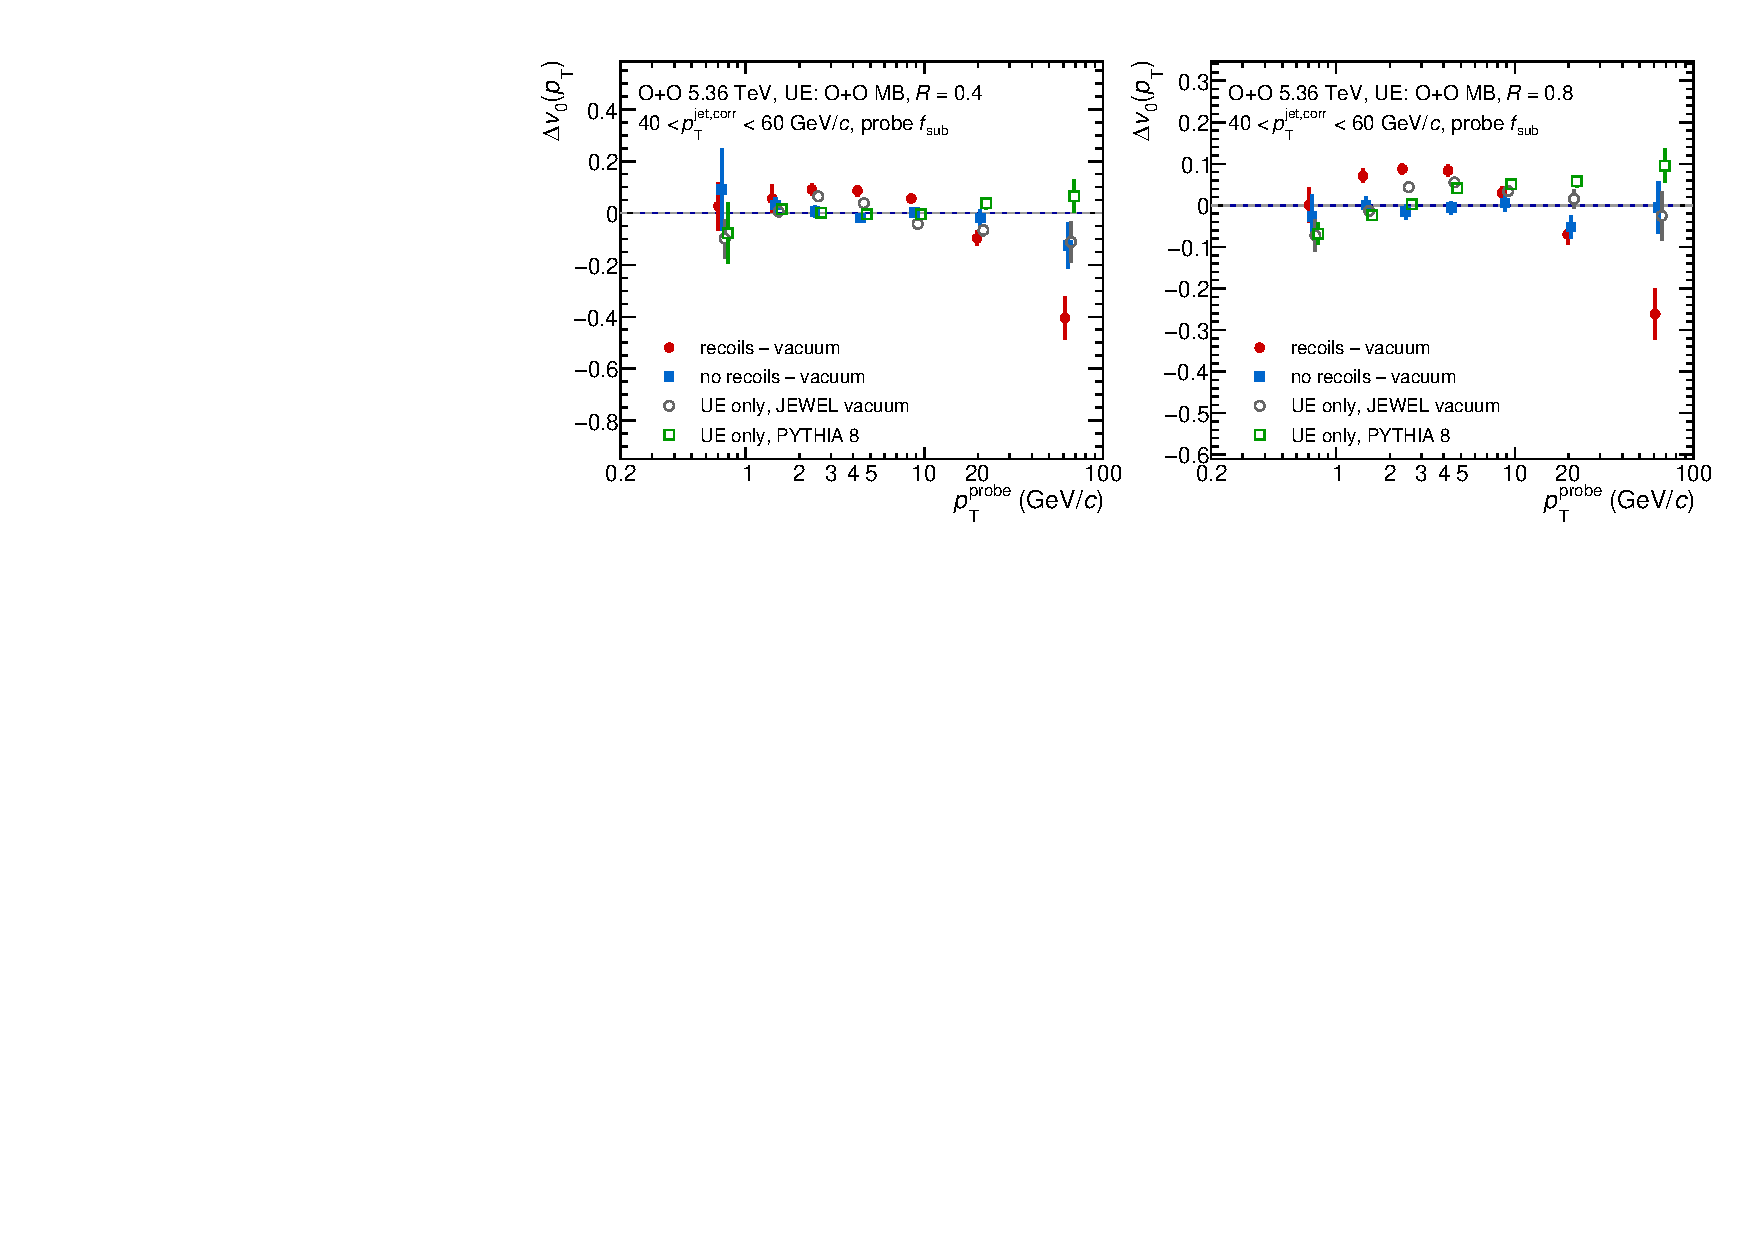
\includegraphics[width=0.98\textwidth]{figs/fig_dv0_pt.pdf}
 \caption{Momentum-dependent change of $\vjet$ for $40<p_{\mathrm T}^{\mathrm{jet,corr}}<60$~GeV/$c$ at the minimum-bias O+O background density, using the perpendicular-cone-subtracted probe. Left and right panels show $R=0.4$ and $0.8$. Red and blue markers compare medium calculations with and without retained recoils to the vacuum sample at the same background level [Eq.~\eqref{eq:signal}]. Open markers show the embedding-induced changes of the two vacuum baselines [Eq.~\eqref{eq:background}]. These are different differences and are displayed together to compare their momentum dependence. Error bars are statistical.}
 \label{fig:dv0pt}
\end{figure*}
The differential changes in Fig.~\ref{fig:dv0pt} reveal the main distinction. The calculation without retained recoils is compatible with the vacuum result in the studied selections; the reported range summaries satisfy $|Z|\le1.2$. Retaining recoils produces a positive change over the soft summary range and a predominantly negative change over the hard range. The latter is unresolved for the smallest cone. Thus the observable responds to the inclusion of recoil particles in this model even when the modification from the no-recoil calculation is not resolved.

This is a change of a correlation, rather than a measurement of the mean recoil yield. A positive $\Delta\vjet$ in the soft range means that the soft-fraction correlation becomes more positive, or less negative, relative to its vacuum value. It does not require the absolute correlation to be positive. Likewise, a negative change at high momentum need not imply an increase of the mean soft yield in every event. Both the numerator and the reference normalization can change when recoils are retained.

Without the additional thermal background, representative modifications are $-0.21\pm0.02$ for hard probes at $R=0.4$ and $+0.095\pm0.003$ for soft probes at $R=0.8$. In this limit the reference contains only activity from the hard event, including the recoil particles (Sec.~\ref{sec:setup}), so these values indicate the sensitivity to the recoils before any dilution by particles unrelated to the jet. The background changes these values but does not eliminate the separation. Table~\ref{tab:signals} gives the results at the minimum-bias O+O background density for $40$--$60$~GeV/$c$ jets. The opposite soft and hard changes are established most clearly for $R\ge0.2$. Their relation to spectral redistribution follows from the normalization of the probe, although the two restricted momentum ranges need not cancel each other: they do not exhaust the probe acceptance and are summarized with uncertainty weights.

\begin{table*}[t]
\caption{Medium-with-recoils minus vacuum at the same minimum-bias O+O background density for $40<p_{\mathrm T}^{\mathrm{jet,corr}}<60$~GeV/$c$, using the perpendicular-cone-subtracted probe. $S$ is the range summary defined in Sec.~\ref{sec:setup}; its quoted uncertainty is statistical. $|Z|$ also includes the baseline terms in Eq.~\eqref{eq:Z}. The $R=0.8$ calculation uses a wider tracking acceptance.}
\label{tab:signals}
\begin{ruledtabular}
\begin{tabular}{ccccc}
$R$ & $S$, $1<\pT<6$ GeV/$c$ & $|Z|$, soft & $S$, $12<\pT<100$ GeV/$c$ & $|Z|$, hard\\
0.1 & $+0.034\pm0.019$ & 1.3 & $+0.008\pm0.018$ & 0.3\\
0.2 & $+0.055\pm0.014$ & 2.1 & $-0.066\pm0.020$ & 1.2\\
0.4 & $+0.086\pm0.015$ & 3.4 & $-0.128\pm0.027$ & 2.0\\
0.8 & $+0.082\pm0.009$ & 5.4 & $-0.097\pm0.024$ & 2.6
\end{tabular}
\end{ruledtabular}
\end{table*}

\subsection{Radius dependence: amplitude and sensitivity}
\begin{figure*}[t]
 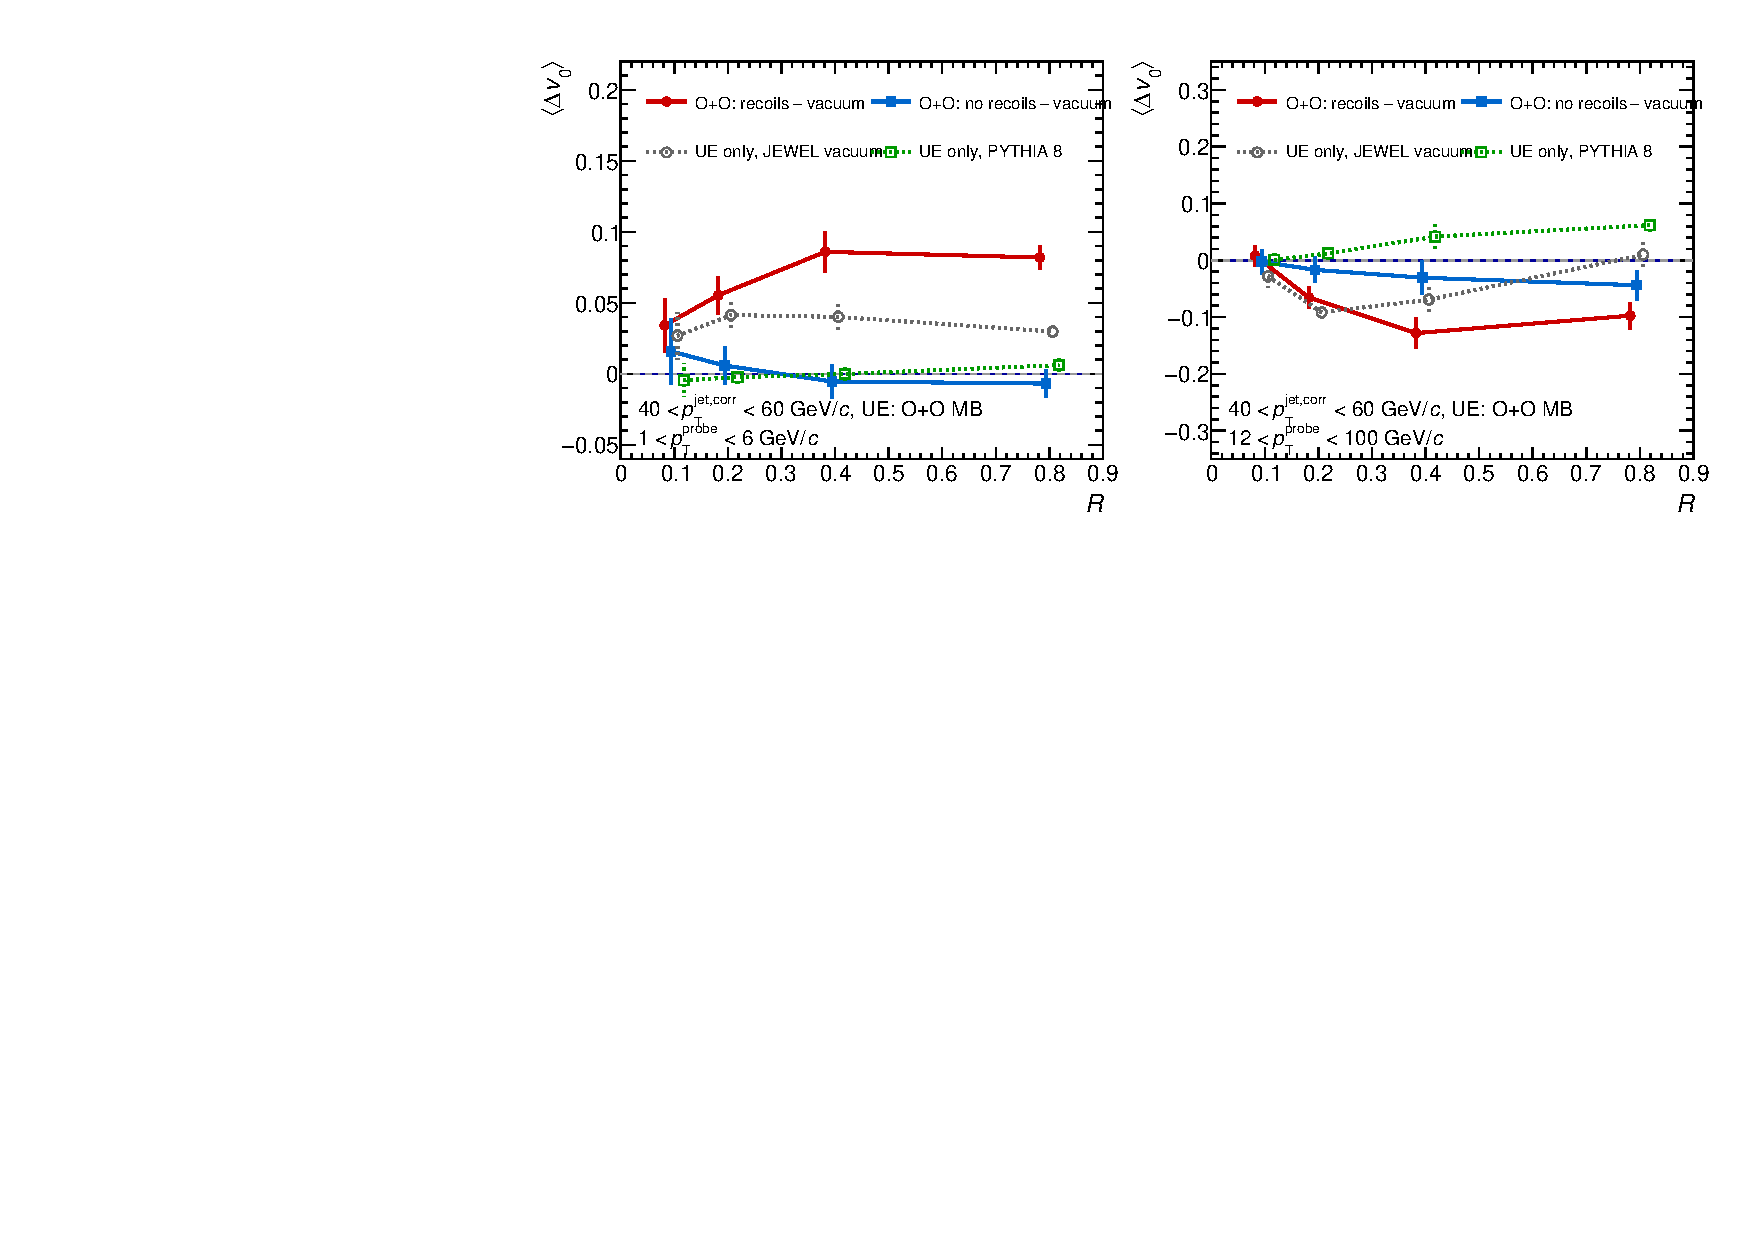
\includegraphics[width=0.98\textwidth]{figs/fig_dv0_R.pdf}
 \caption{Radius dependence of the changes in $\vjet$ for $40<p_{\mathrm T}^{\mathrm{jet,corr}}<60$~GeV/$c$ at the minimum-bias O+O background density. Left: the soft range $1<\pT<6$~GeV/$c$. Right: the hard range $12<\pT<100$~GeV/$c$. Range averages use inverse statistical-variance weights. The medium differences and the two vacuum embedding differences follow Eqs.~\eqref{eq:signal} and \eqref{eq:background}. The tracking acceptance changes from $|\eta|<0.9$ to $|\eta|<2.5$ at $R=0.8$. Error bars are statistical.}
 \label{fig:radius}
\end{figure*}
The soft modification increases from $R=0.1$ to $0.4$ and is comparable at $R=0.8$ (Fig.~\ref{fig:radius}). The central values therefore do not show a monotonically increasing amplitude over the full radius range. In contrast, the sensitivity diagnostic increases from $1.3$ to $5.4$, reflecting the signal, statistical uncertainty, and background-baseline uncertainty together. The smaller error at $R=0.8$ contributes to its greater sensitivity.

The changes between neighboring radii are about $0.02$--$0.03$ in the soft range between $R=0.1$ and $0.4$, and are individually only about $1$--$1.5$ times their quadrature statistical uncertainties. They do not localize the response in an annulus. The larger cone changes which particles belong to the probe and reference; the $R=0.8$ point also uses a larger pseudorapidity acceptance. A fixed-acceptance scan with correlated uncertainties is required before assigning a characteristic angular scale to the response. The present comparison identifies favorable analysis configurations within the studied selections.

The hard-probe baseline deserves particular attention for lower-momentum, large-radius jets. For $20$--$40$~GeV/$c$ jets at $R=0.8$, the embedding-induced change is $+0.33\pm0.15$ in JEWEL vacuum and $+0.27\pm0.03$ in PYTHIA, while the medium-with-recoils difference at matched background is $-0.64\pm0.16$. The opposite signs help distinguish the medium modification from the embedding effect in these calculations. The reported diagnostic is $|Z|=3.6$. Agreement of two vacuum models constrains this particular baseline estimate; it does not provide a complete uncertainty on the physical UE.

\subsection{Subtraction, reference selection, and normalization}
\begin{figure*}[t]
 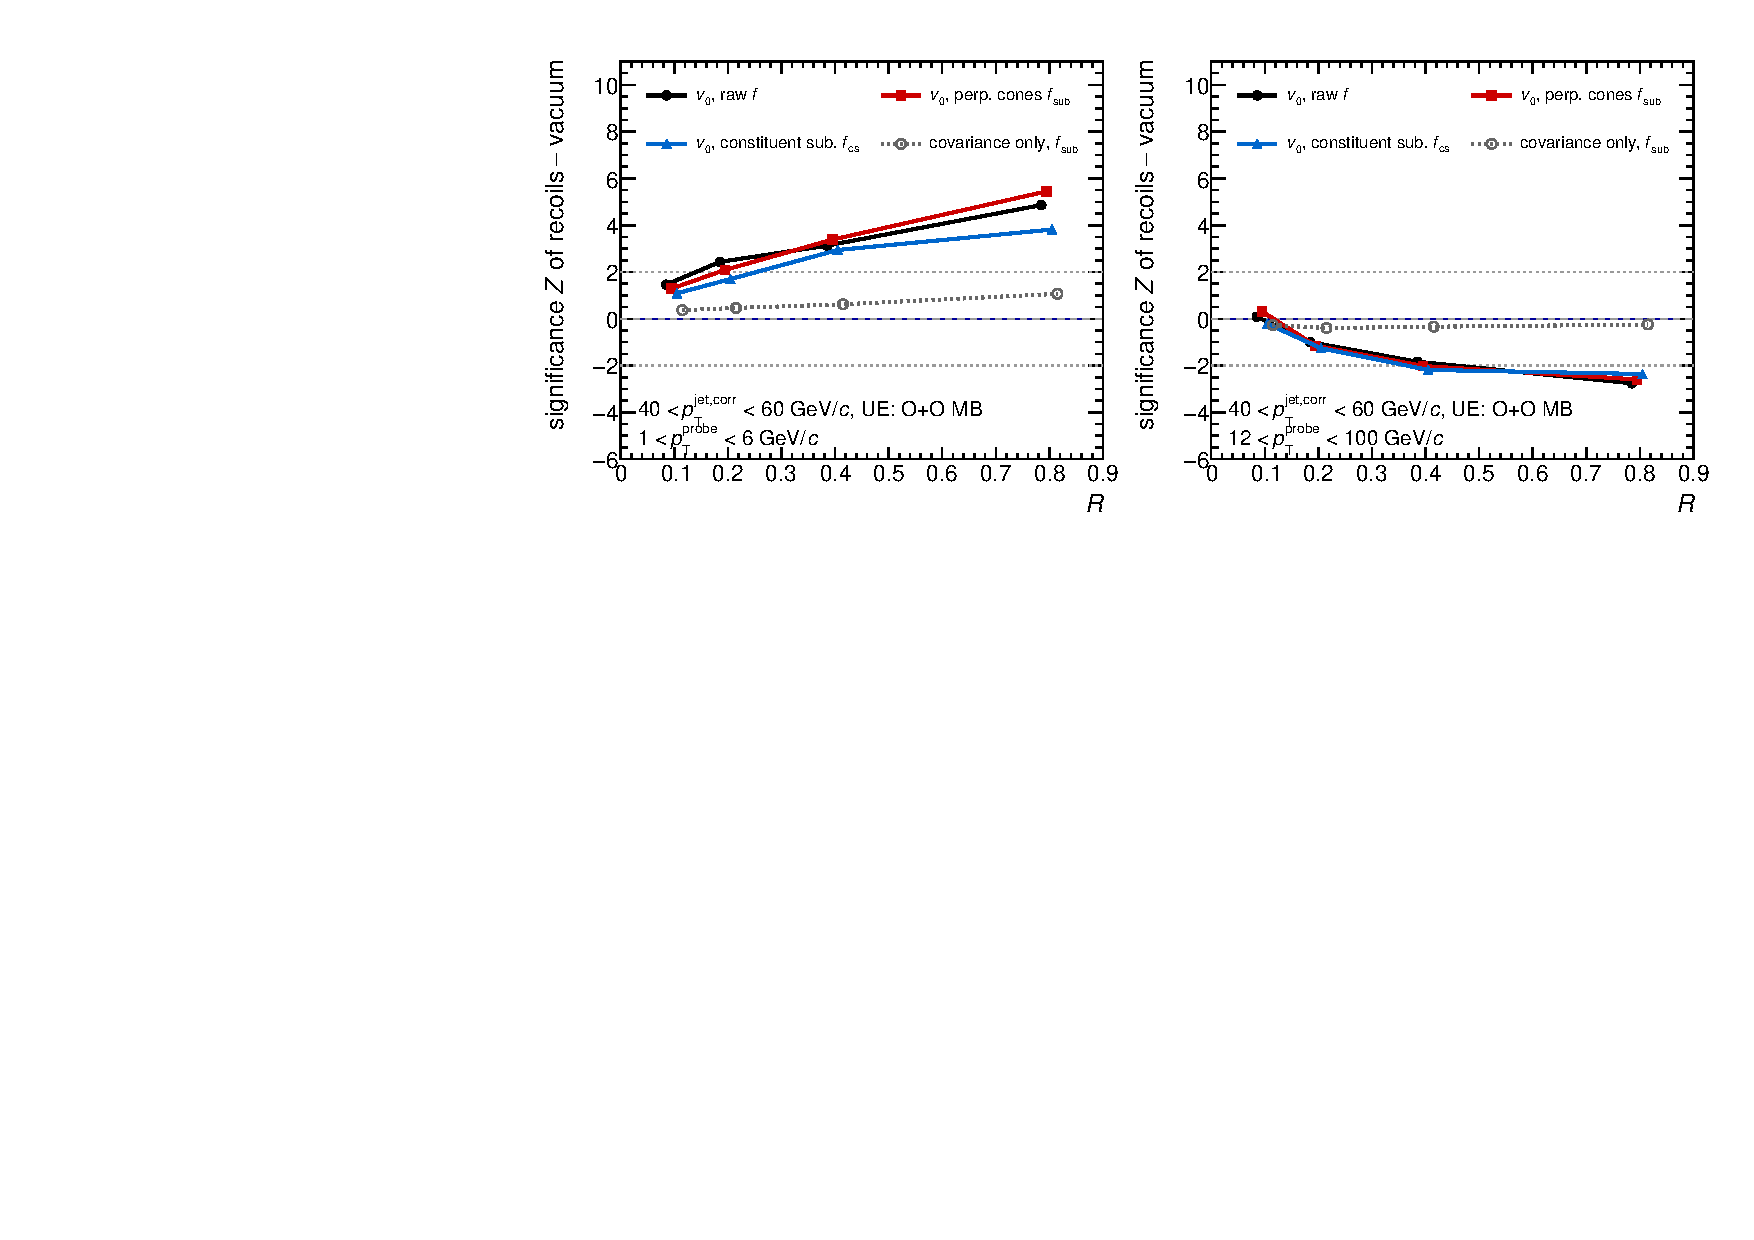
\includegraphics[width=0.98\textwidth]{figs/fig_methods.pdf}
 \caption{Signed sensitivity diagnostic $Z$ [Eq.~\eqref{eq:Z}] for the recoil-retaining medium difference, versus $R$, for $40<p_{\mathrm T}^{\mathrm{jet,corr}}<60$~GeV/$c$ and the minimum-bias O+O background density. Left: soft probes. Right: hard probes. The raw, perpendicular-cone-subtracted, and constituent-subtracted spectra are compared with the unnormalized covariance. These values characterize the generated samples and the assigned baseline uncertainty; they are not experimental discovery projections.}
 \label{fig:vsR}
\end{figure*}
Figure~\ref{fig:vsR} compares the full estimator for three probe definitions. The soft response at $R=0.8$ gives $Z=4.9$, $5.4$, and $3.8$ for the raw, perpendicular-cone-subtracted, and constituent-subtracted spectra, respectively. For hard probes at $R=0.4$, the corresponding magnitudes are $1.8$, $2.0$, and $2.2$. The common sign and qualitative separation support the result across these subtraction choices. Similar values of $Z$ alone do not establish equality of the underlying signal amplitudes or demonstrate complete subtraction closure.

The reference-gap selection gives reported sensitivities of $|Z|=4.9$ and $4.0$ for soft and hard probes at $R=0.8$, while the values at $R\le0.4$ are below two. This variation tests the dependence on the reference region, but also changes its multiplicity and fluctuation scale. In particular, persistence with a gap is not sufficient to establish a collective origin: wide-angle recoil activity and event-selection correlations can survive the gap.

Varying the thermal-momentum subtraction distance in the recoil calculation from $1.0$ to $0.5$ changes the reported signal by less than $0.02$. Omitting thermal subtraction shifts the soft-range result by at most $0.04$ and the hard-range result at $R=0.4$ by $-0.09\pm0.02$, comparable to the nominal hard signal. The latter comparison illustrates contamination by the original thermal momenta, which are not energy deposited by the jet. Complete omission is not an equally valid subtraction prescription. Stability under the distance variation is therefore the more relevant robustness test, while the omission test shows why thermal subtraction is necessary.

The reference normalization has a measurable impact. For the bare covariance $\Cov(f_b,\mpt)$, the reported diagnostic satisfies $|Z|\le1.1$ in the studied selections. Its embedding-induced change is several times the medium difference. Dividing by $\sqrt{\Ctwo}$ substantially reduces this dominance in the present samples. The restricted independent-background limit in Appendix~\ref{app:dilution} explains how such a cancellation can occur. Residual composition effects, changes of the probe, and selection effects remain, as demonstrated by the nonzero $F_g$. The empirical improvement of the normalized estimator is a result of this study, not a general theorem that it is immune to the UE.

\section{Discussion and outlook}\label{sec:discussion}
The novel information carried by $\vjet$ is the covariance between redistribution of particles inside a selected jet and changes of the surrounding mean momentum. This information is absent from an average fragmentation spectrum. It is also different from the angular, energy-weighted information in a conventional EEC. The observable connects a method developed for bulk momentum fluctuations to a jet-conditioned measurement while retaining a transparent normalization constraint.

The JEWEL comparison provides a specific demonstration of response sensitivity. For the tested selections, including retained recoils produces a modification that is not resolved in the corresponding calculation without recoils. This is useful discrimination within a common model setup, but does not imply that every energy-loss model without an explicit recoil component gives zero modification. Changes of fragmentation, quark/gluon composition, jet selection, and reference activity can all affect the measured covariance. A calculation that reproduces both the baseline and its medium modification is needed to assess these possibilities.

Several features guide a measurement. The soft range gives the largest separation under the stated prescription. Large-radius configurations retain sensitivity at the minimum-bias O+O background density, including with a more separated reference. The normalized observable is substantially more effective than its bare covariance in this embedding test. These findings favor a differential measurement across probe momentum and reference selections, accompanied by vacuum embedding controls. They do not yet establish an optimal radius, since acceptance and reconstruction differ across the scan.

The reconstruction checks in Appendix~\ref{app:qa} identify limitations that matter for this interpretation. The lowest momentum bins do not exhibit complete subtraction closure, and the $R=0.8$ area-corrected selection has a residual momentum shift. A dedicated experimental analysis would need to propagate these effects, detector response, the joint covariance of the baseline subtraction, and the available event statistics. The model-spread term from two vacuum generators should be supplemented by variations of background fluctuations and correlations, not interpreted as covering all UE uncertainty.

The relation to radial flow remains a physics opportunity rather than a demonstrated conclusion. The present background is independent and JEWEL retains microscopic recoils without evolving their coupling to collective expansion. Calculations with a hydrodynamic response and a correlated bulk event can test whether equilibration generates additional momentum, species, or reference-gap dependence. Measuring identified probe particles and using fixed-jet angular reference intervals would extend the information available beyond the present integrated reference. A joint comparison with EECs could then constrain the same candidate response model through different momentum weights and geometrical selections.

\section{Summary}\label{sec:summary}
We have proposed a normalized jet--UE transverse-momentum correlation that measures how the in-cone spectral shape varies with the mean momentum outside the cone. Its leading pair representation contains a bin weight with the mean fraction subtracted and a reference momentum measured relative to its mean. These weights distinguish it from energy correlators and explain its sensitivity to particle redistribution. Exact ratio corrections and the conditions for cancellation of independent-background dilution have been stated explicitly.

In JEWEL O+O calculations at $5.36$~TeV, retaining recoils generates positive soft-probe and predominantly negative hard-probe modifications, while the no-recoil calculation remains compatible with the vacuum baseline. The soft amplitude increases up to $R=0.4$ and is comparable at $R=0.8$; its sensitivity increases to $Z=5.4$ in the latter configuration under the specified simulated-sample uncertainty prescription. The separation persists across the tested probe subtraction methods, and reference normalization improves the separation relative to the bare covariance. These results motivate a measurement of jet--UE spectral correlations and further calculations that connect microscopic recoil response to the collective evolution of the medium.

\bibliography{refs}

% Add acknowledgments and funding statements after author verification.
\appendix
\section{Exact ratios and connected pair representation}\label{app:derivation}
The distinction between a mean of ratios and a ratio of means follows directly from Eq.~\eqref{eq:residuals}:
\begin{equation}
 f_b=\bar f_b+\frac{\Delta n_b}{N},\qquad
 \mpt=\bar p_{\mathrm{ref}}+\frac{\Delta P_{\mathrm{ref}}}{M}.
\end{equation}
Since $\av{\Delta n_b}=\av{\Delta P_{\mathrm{ref}}}=0$, but the denominators fluctuate, the exact covariance is
\begin{align}
 \Cov(f_b,\mpt)={}&\av{\frac{\Delta n_b\Delta P_{\mathrm{ref}}}{NM}}
 -\av{\frac{\Delta n_b}{N}}\av{\frac{\Delta P_{\mathrm{ref}}}{M}}.
 \label{eq:exact}
\end{align}
Expanding the reciprocal denominators gives
\begin{align}
 \Cov(f_b,\mpt)={}&\frac{\av{\Delta n_b\Delta P_{\mathrm{ref}}}}{\av N\av M}
 -\frac{\av{\Delta n_b\Delta P_{\mathrm{ref}}\delta N}}{\av N^2\av M}\nonumber\\
 &-\frac{\av{\Delta n_b\Delta P_{\mathrm{ref}}\delta M}}{\av N\av M^2}
 +\mathcal O(\delta^4).
 \label{eq:corrections}
\end{align}
The notation $\mathcal O(\delta^4)$ counts powers of fluctuations, not particle order. The leading term contains two powers; the displayed corrections contain three. The second term of Eq.~\eqref{eq:exact}, a product of residual-ratio means, begins at fourth order. No universal $1/N$ error estimate follows without assumptions about these joint moments.

For arbitrary additive sums $A=\sum_i a(x_i)$ and $B=\sum_j b(x_j)$, separating the equal-index terms gives
\begin{align}
 \Cov(A,B)={}&\iint\dd x_1\dd x_2\,a(x_1)b(x_2)C(x_1,x_2)\nonumber\\
 &+\int\dd x\,a(x)b(x)\rho_1(x).
 \label{eq:additive}
\end{align}
For disjoint regions, the same-particle term on the second line is zero. Applying this identity to the residuals gives Eq.~\eqref{eq:corr}. The identity for additive sums is exact; the approximation originates in replacing the fluctuating denominators. A direct comparison of Eq.~\eqref{eq:fourterms} with the measured covariance tests its accuracy for a given sample. The observable itself should still be evaluated from Eq.~\eqref{eq:v0}.

\section{Independent-background dilution and its limits}\label{app:dilution}
Consider an illustrative reference made of $M_{\mathrm s}$ particles from the original jet event and $M_{\mathrm u}$ added particles. Define their event means $q_{\mathrm s}$ and $q_{\mathrm u}$ and the event fraction $\alpha_e=M_{\mathrm s}/(M_{\mathrm s}+M_{\mathrm u})$. The exact reference mean is
\begin{equation}
 \mpt=\alpha_e q_{\mathrm s}+(1-\alpha_e)q_{\mathrm u}.
 \label{eq:mixture}
\end{equation}
Take a fixed probe and selection and an independently added component. To leading order, with $\alpha=\av{M_{\mathrm s}}/\av M$ and component centering momenta $\bar p_{\mathrm s}$ and $\bar p_{\mathrm u}$,
\begin{align}
 \Cov(f_b,\mpt)\simeq{}&\alpha\Cov(f_b,q_{\mathrm s})\nonumber\\
 &+\frac{(1-\alpha)(\bar p_{\mathrm s}-\bar p_{\mathrm u})}{\av M}
 \Cov(f_b,M_{\mathrm s}).
 \label{eq:composition}
\end{align}
Here independence sets the corresponding covariances with the added mean and count to zero. The second term is a composition effect: changing the mixture changes the reference mean when the two components have different mean momenta. Reconstructed-jet selection or a multiplicity condition involving both components can invalidate the required independence even when embedding was initially independent.

A particularly transparent limit fixes both component counts, sets their mean momenta equal, takes the added particles to have no distinct-pair correlation, and leaves the probe unchanged. Then
\begin{align}
 \Cov(f_b,\mpt)&=\alpha\Cov(f_b,q_{\mathrm s}),\nonumber\\
 C_{2,\mathrm{ref}}&=\frac{M_{\mathrm s}(M_{\mathrm s}-1)}{M(M-1)}C_{2,\mathrm s}.
 \label{eq:fixeddilution}
\end{align}
Thus the covariance is diluted by the single-particle fraction and the pair correlator by the distinct-pair fraction. Their ratio satisfies
\begin{equation}
 \frac{\vjet_{\mathrm s+u}(b)}{\vjet_{\mathrm s}(b)}
 =\sqrt{\frac{M_{\mathrm s}(M-1)}{M(M_{\mathrm s}-1)}},
 \label{eq:finitecount}
\end{equation}
for nonzero numerator and $M_{\mathrm s}>1$. It approaches unity at large counts; the finite-count result is not exactly one. Fluctuating component counts, unequal component means, correlations within the bulk, and changes of the probe or selection introduce additional terms. The observed reduction of background sensitivity must therefore be established by embedding and closure checks, not assumed from an exact cancellation.

\section{Jet reconstruction and supplementary checks}\label{app:qa}
The supplementary distributions document reconstruction and estimator behavior. The event-record checks use a subset of 20 output files per sample, corresponding to approximately $4\times10^5$ events. They supplement the correlation analysis and are not a new independent determination of its uncertainties.

Figures~\ref{fig:evd_antikt} and \ref{fig:evd_cs} illustrate the reconstruction steps on single events, using the same code path as the production analysis. They show one PYTHIA event with the minimum-bias thermal background and one JEWEL O+O event with retained recoils. Figure~\ref{fig:evd_antikt} shows the anti-$k_t$ clustering, the leading-jet selection, the perpendicular-cone estimate, and the probe fractions. Figure~\ref{fig:evd_cs} shows the event-wise constituent subtraction and the subtraction of the thermal momenta of the scattering centres. A single event demonstrates the procedure; it does not characterize its average performance, which is assessed in the following figures.

Figure~\ref{fig:qa_jets} compares corrected jet spectra, jet areas, and event-matched momentum residuals after embedding. The area is evaluated with ghosts of area $0.05$, producing visible discretization in the area distribution. At $R=0.4$, both corrections leave a mean shift near $-1$~GeV/$c$, with widths of about $2.3$--$4.1$~GeV/$c$. At $R=0.8$, the area correction leaves shifts near $-4$ to $-5$~GeV/$c$, whereas constituent subtraction stays approximately within $1$~GeV/$c$. A negative residual means that selecting a fixed corrected momentum can preferentially retain harder original jets. The residual shift must therefore enter the interpretation of the large-radius comparison.

Figure~\ref{fig:qa_spectra} compares the reference spectrum without embedding to raw and subtracted spectra after embedding. Above approximately $2$~GeV/$c$, both methods approach the unembedded result. Below $1$--$2$~GeV/$c$, perpendicular-cone subtraction tends to undershoot it and constituent subtraction to overshoot it. The $1$~GeV/$c$ lower edge of the soft summary reduces the influence of the lowest bins, but does not remove the imperfect closure in the $1$--$2$~GeV/$c$ interval. The spread of subtraction methods is therefore a relevant control, not a proof that this interval is unbiased.

Figures~\ref{fig:qa_reference} and \ref{fig:qa_gap} show the reference mean, pair correlator, and reference-gap variation. Figure~\ref{fig:qa_radius} shows differences of the signal between successive radii. The plotted difference errors add the separate-radius errors in quadrature. Shared events can correlate the two estimates, but the sign of that covariance has not been established by these plots; the quadrature error is not necessarily conservative. Figure~\ref{fig:qa_fraction} compares mean normalized spectra, Fig.~\ref{fig:qa_closure} shows the change of the full estimator after vacuum embedding, and Fig.~\ref{fig:qa_recoil} tests the treatment of thermal recoil momenta. In particular, vacuum embedding does not give exact closure of $\vjet$, especially for large radii and harder probes. This motivates the explicit $F_g$ baseline.

\begin{figure*}[tp]
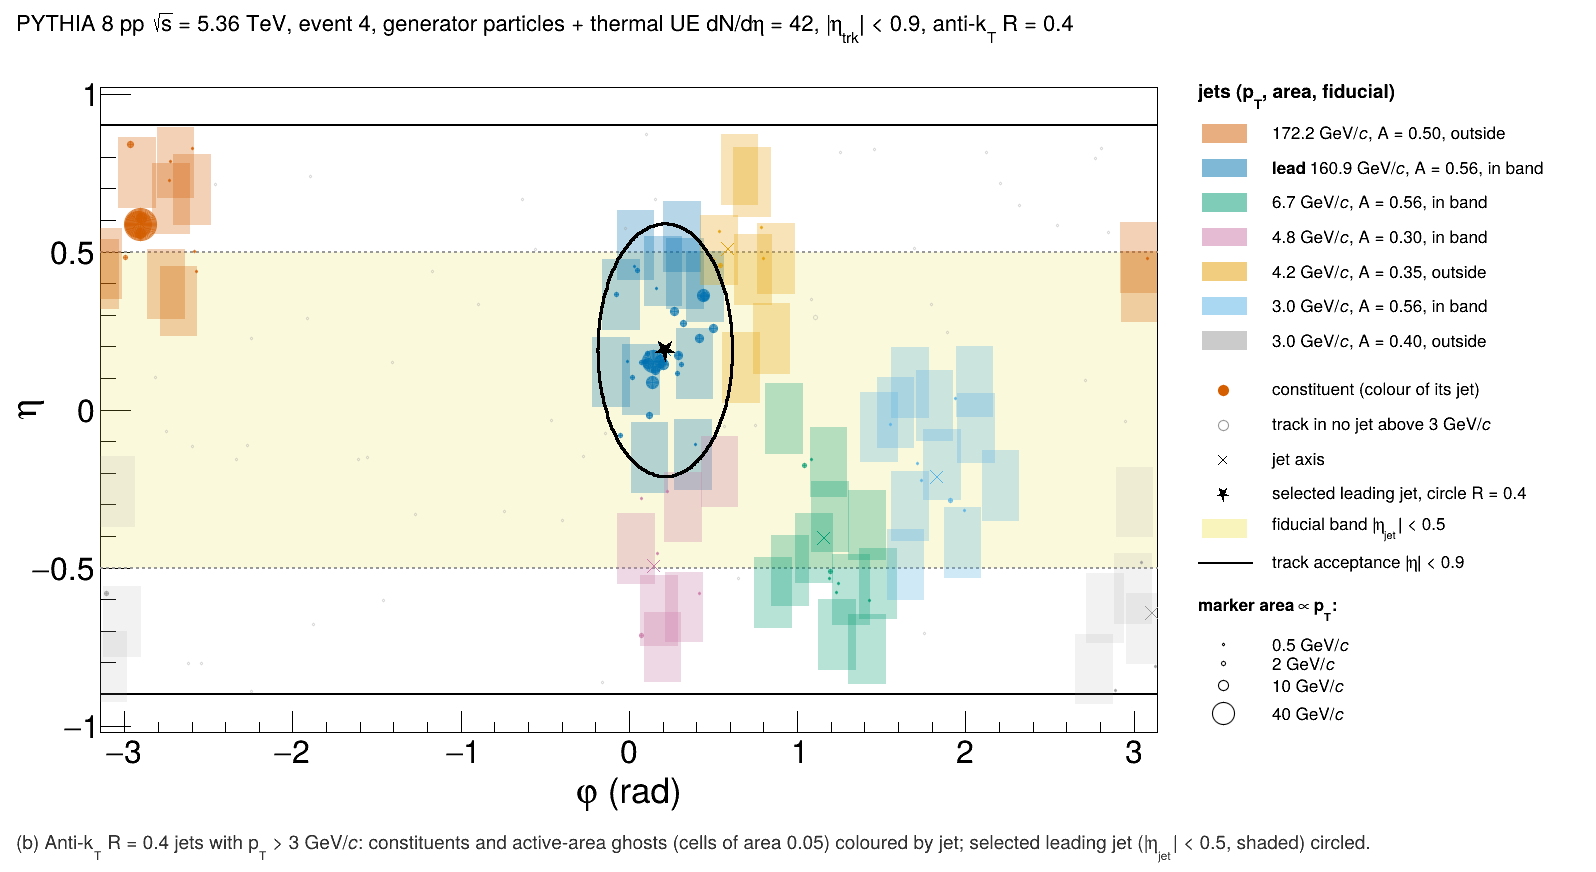
\includegraphics[width=0.88\textwidth]{figs/evd_antikt.png}\\[1mm]
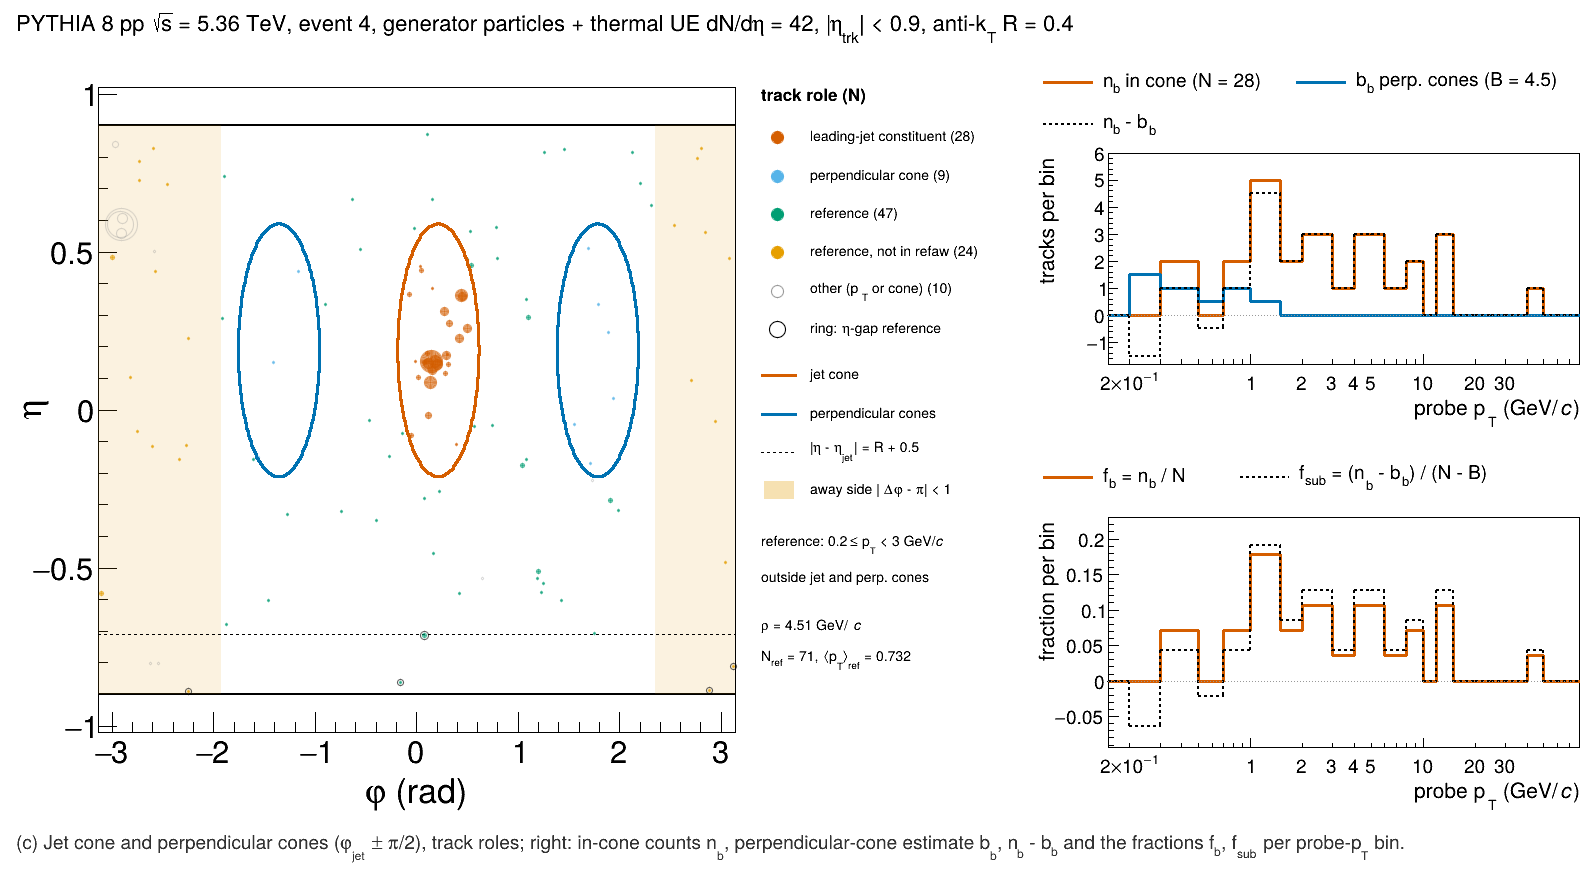
\includegraphics[width=0.88\textwidth]{figs/evd_perpcone.png}
\caption{Jet reconstruction and perpendicular-cone subtraction in one event. Top: Anti-$k_t$ clustering with $R=0.4$ for one PYTHIA~8 pp event with the minimum-bias thermal background added ($\dd N_{\mathrm{ch}}/\dd\eta=42$). Charged particles with $\pT>0.15$~GeV/$c$ and $|\eta|<0.9$ are clustered. Jets above $3$~GeV/$c$ are shown by their constituents and by the active-area ghosts assigned to them, both coloured by jet; the marker area is proportional to $\pT$. The leading jet is selected among jets with $|\eta_{\mathrm{jet}}|<0.9-R$ (shaded band); here the highest-momentum jet lies outside this band, so the next jet is selected (circle). The legend lists each jet's momentum, area, and fiducial status. Bottom: Perpendicular-cone estimate and probe fractions for the same event. Left: the jet cone, the two cones at $\varphi_{\mathrm{jet}}\pm\pi/2$, and the role of each track: jet constituent, perpendicular cone, nominal reference ($0.2<\pT<3$~GeV/$c$ outside the jet and perpendicular cones), the part of the reference removed by the away-side exclusion $|\Delta\varphi-\pi|<1$ (shaded), and tracks entering the pseudorapidity-gap reference (ringed). Right, top: in-cone counts $n_b$, the background estimate $b_b$ averaged over the two perpendicular cones, and $n_b-b_b$. Right, bottom: the raw fraction $f_b$ and the subtracted fraction $f_{b,\mathrm{sub}}$ of Eq.~\eqref{eq:subtracted}. Bins with $n_b<b_b$ give negative subtracted contents.}
\label{fig:evd_antikt}
\end{figure*}

\begin{figure*}[tp]
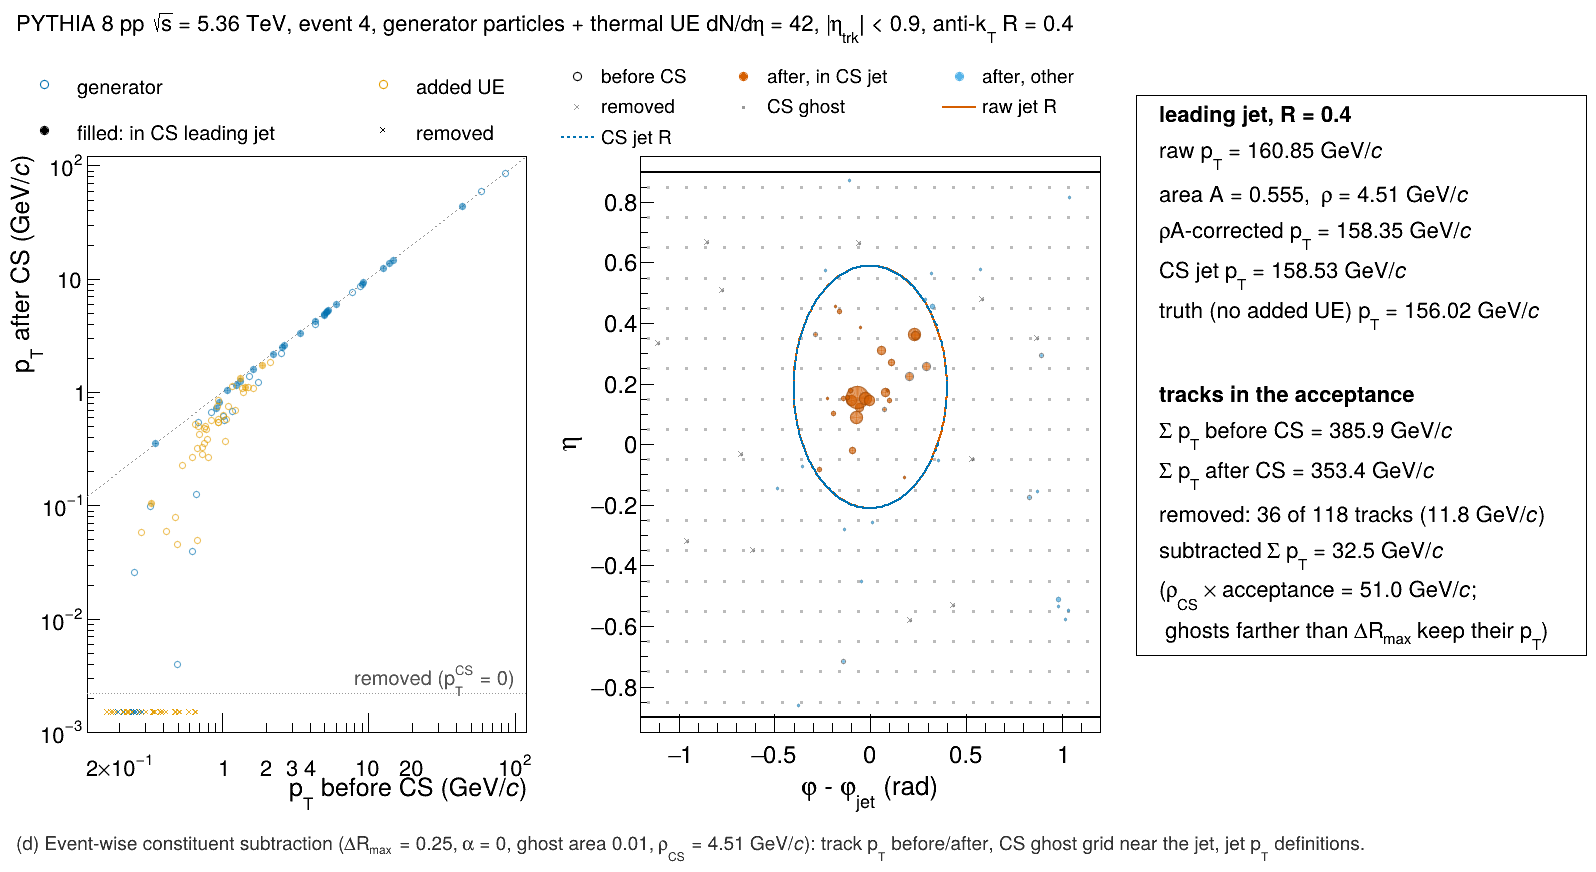
\includegraphics[width=0.88\textwidth]{figs/evd_cs.png}\\[1mm]
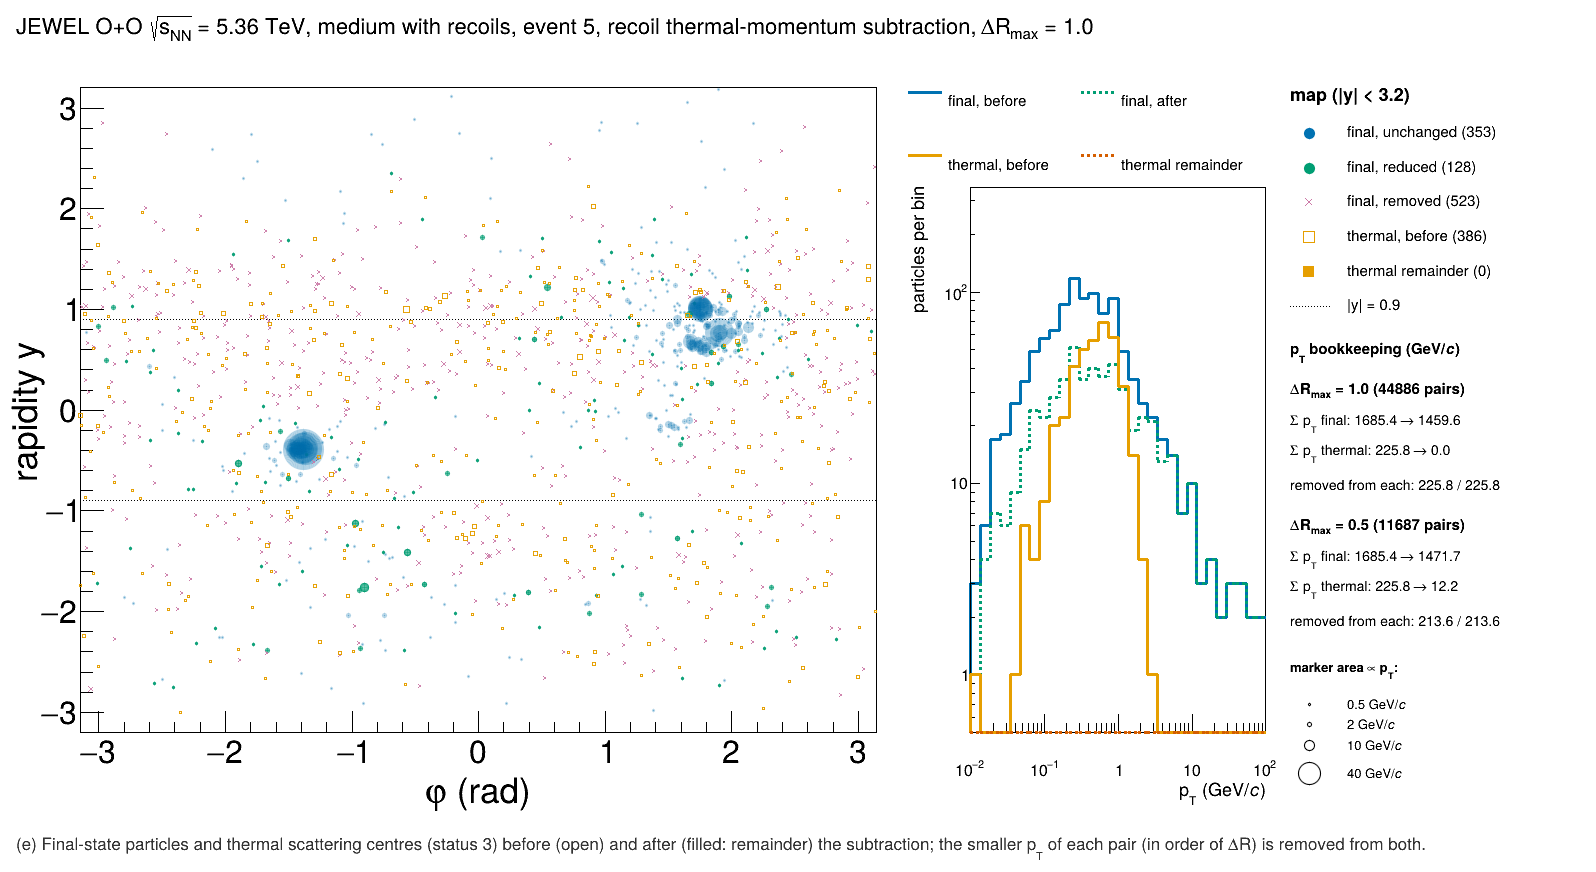
\includegraphics[width=0.88\textwidth]{figs/evd_recoil.png}
\caption{Constituent subtraction and recoil thermal-momentum subtraction. Top: Event-wise constituent subtraction for the event of Fig.~\ref{fig:evd_antikt}. Left: track momentum after versus before subtraction, separately for generator particles and added background; removed tracks are shown at the bottom. Middle: tracks after subtraction near the jet, the ghosts carrying the background density $\rho$, and the raw and subtracted jet boundaries. Right: the leading-jet momentum before correction, after the area correction of Eq.~\eqref{eq:jetcorr}, after constituent subtraction, and the corresponding jet in the same event without added background, together with the total subtracted momentum. Bottom: Subtraction of the thermal momenta of the scattering centres in one JEWEL O+O event with retained recoils. Left: final-state particles that are unchanged, reduced, or removed by the subtraction, and the thermal momenta (open squares) that are subtracted. Right: momentum distributions before and after the subtraction, and the bookkeeping of the subtracted momentum for maximum matching distances $1.0$ (nominal) and $0.5$. Pairs are processed in order of increasing distance, and the smaller momentum of each pair is removed from both members. A reduced final-state particle is a particle whose momentum was lowered by this procedure; hadron-level recoil particles cannot be identified individually.}
\label{fig:evd_cs}
\end{figure*}

\begin{figure*}[tp]
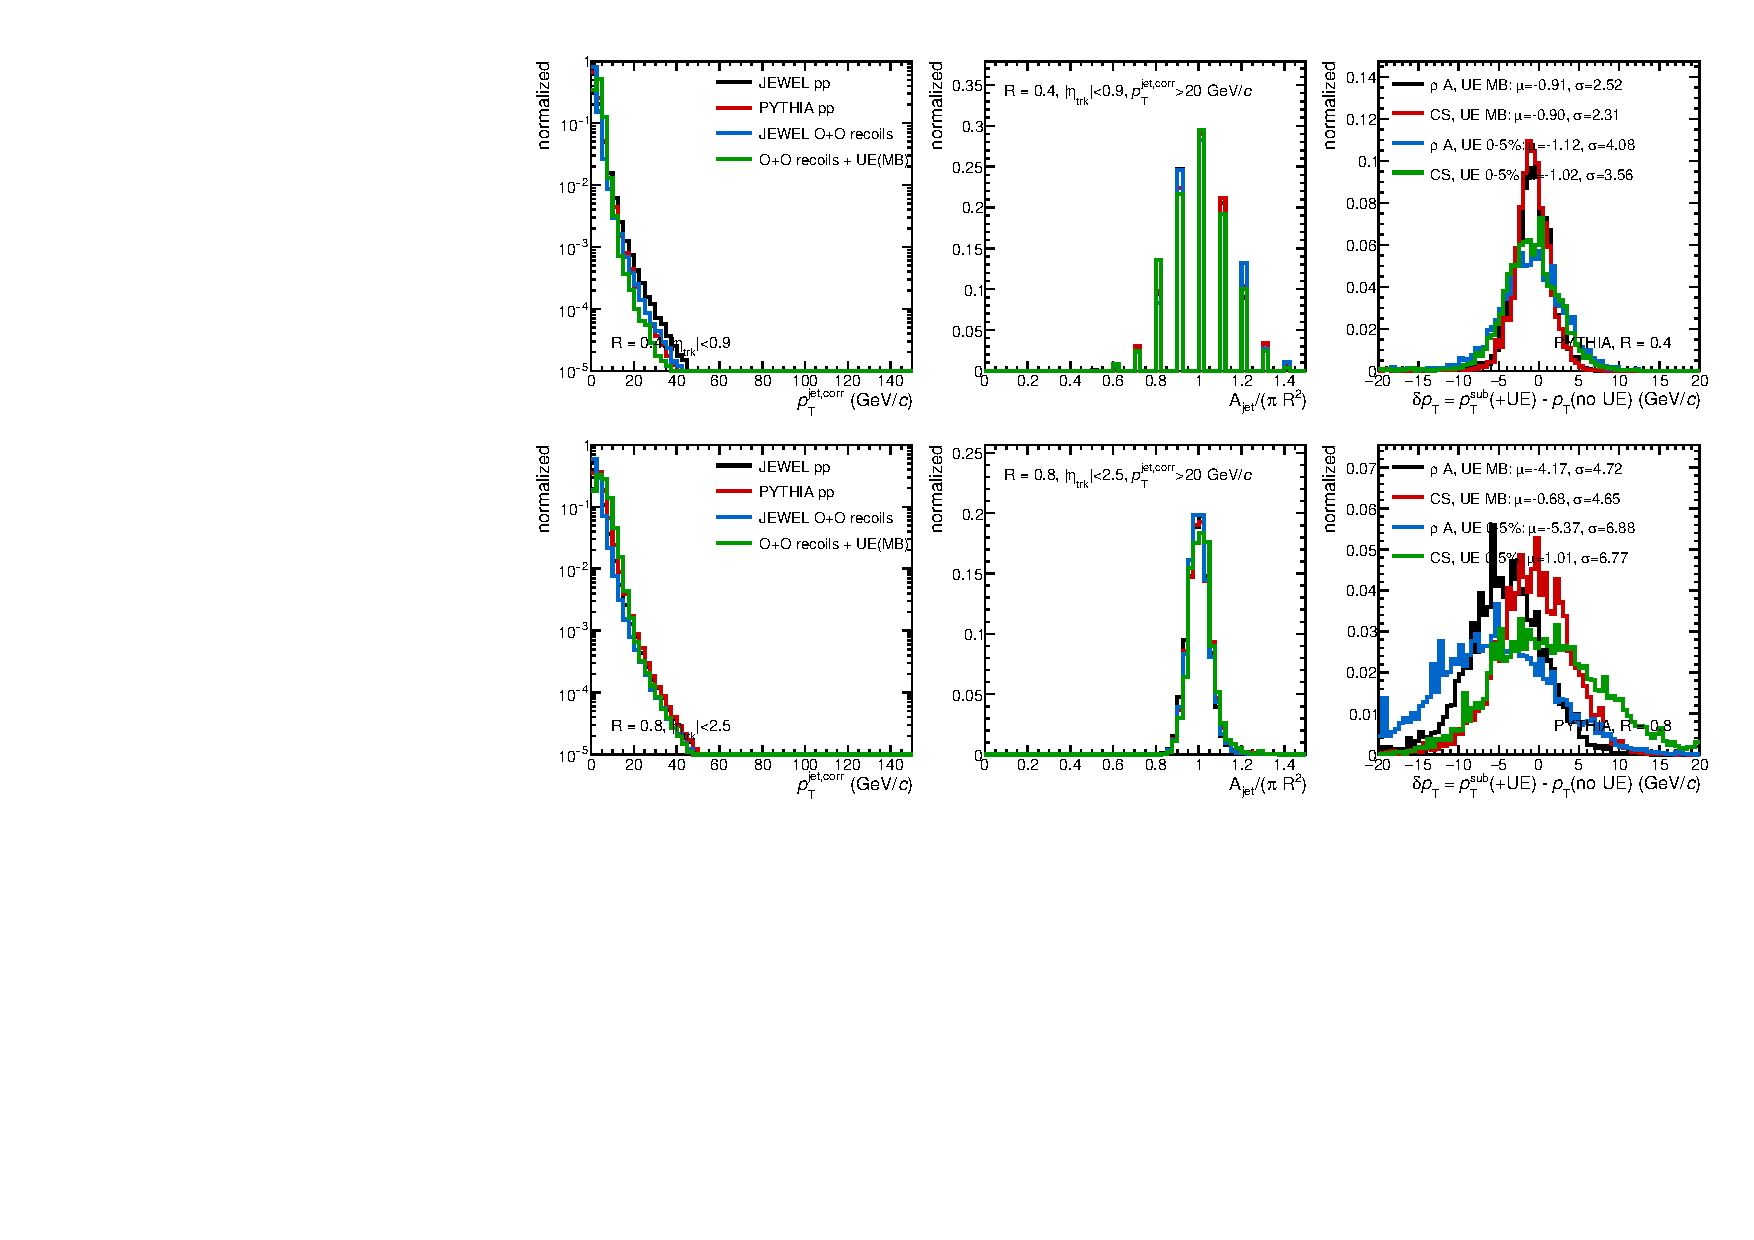
\includegraphics[width=0.98\textwidth]{figs/qa_jets.pdf}
\caption{Jet reconstruction checks for $R=0.4$ (top) and $0.8$ (bottom). Left: normalized corrected leading-jet momentum spectra. Middle: area divided by $\pi R^2$ for corrected jet momentum above $20$ GeV/$c$. Right: event-matched residual momentum after background correction relative to the corresponding unembedded jet. Legends give the mean and width for area and constituent subtraction at the two embedding densities.}
\label{fig:qa_jets}
\end{figure*}

\begin{figure*}[tp]
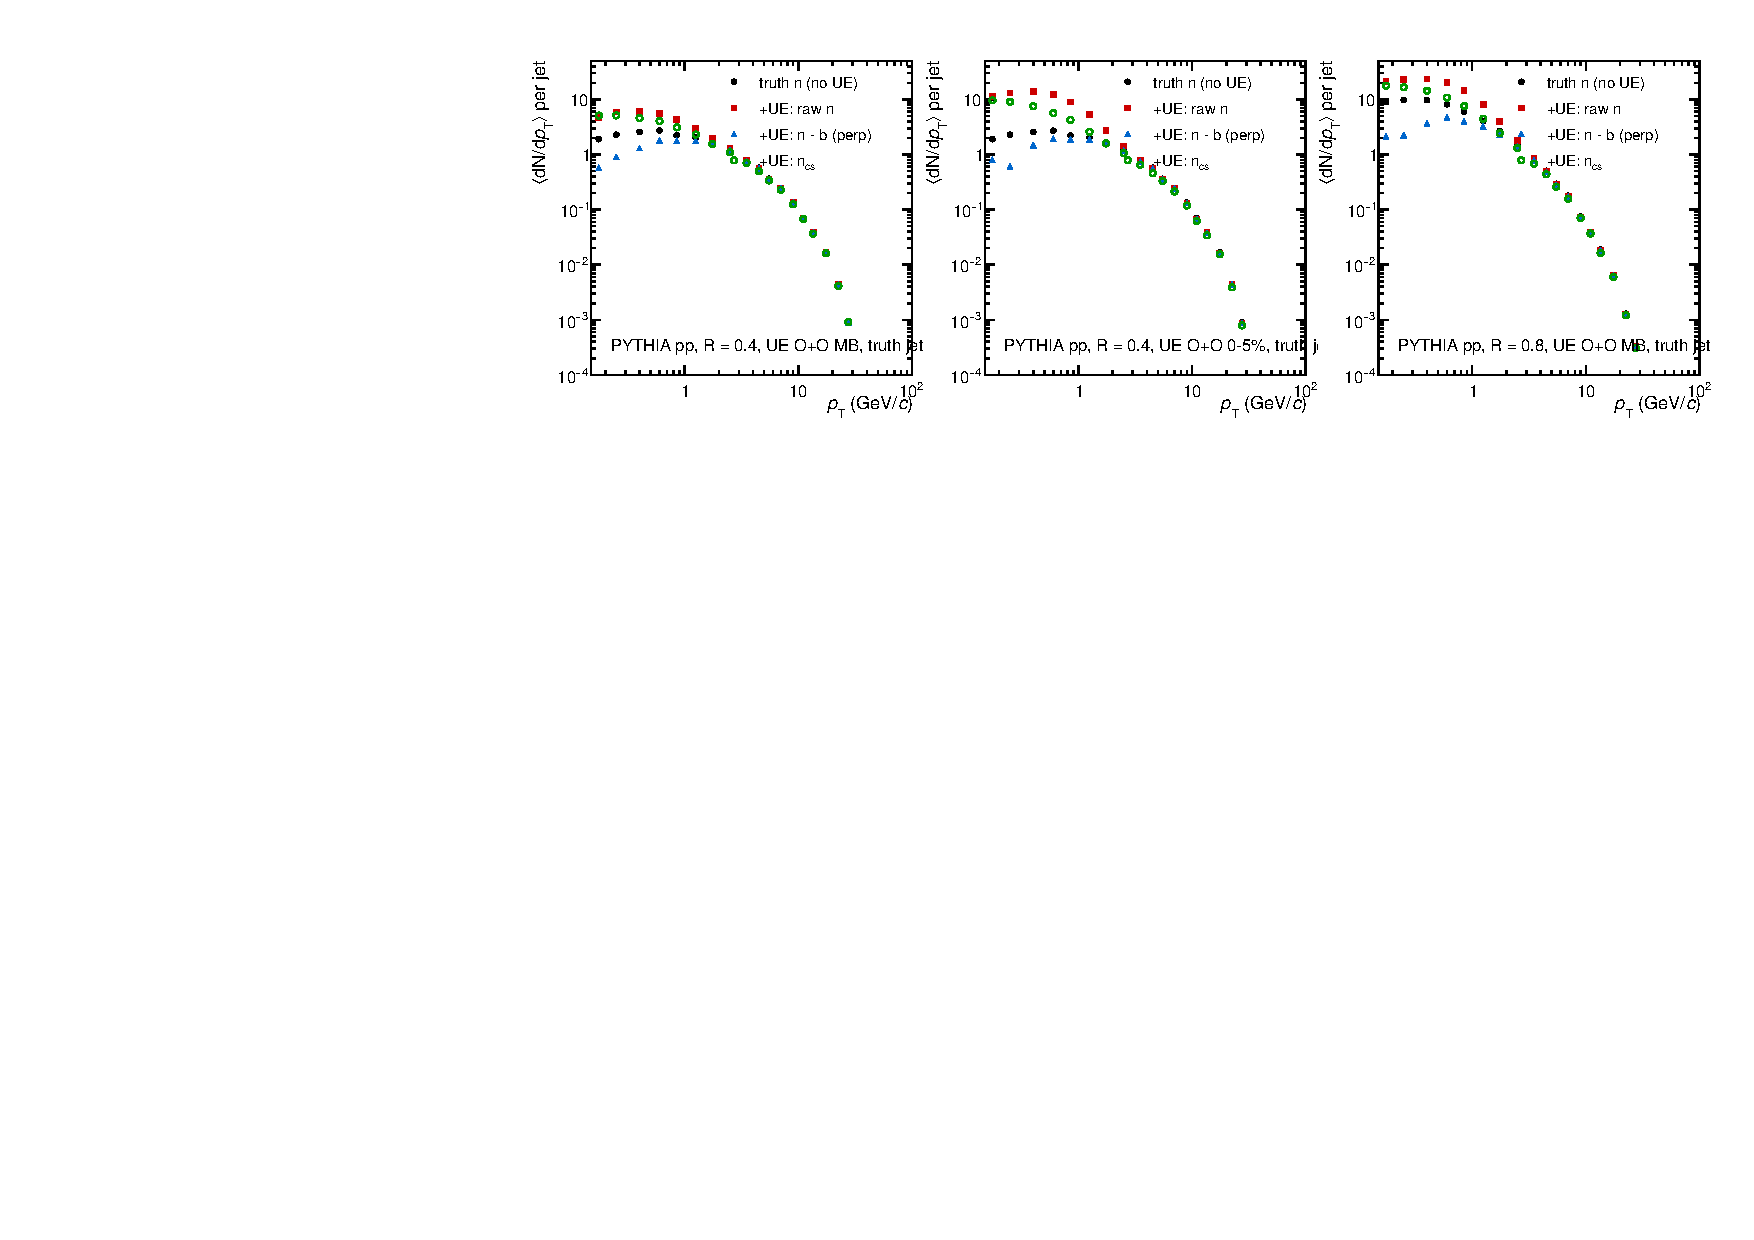
\includegraphics[width=0.98\textwidth]{figs/qa_spectra.pdf}
\caption{Charged-particle spectra per jet in PYTHIA, comparing the unembedded spectrum with raw, perpendicular-cone-subtracted, and constituent-subtracted spectra after embedding. Panels show the indicated radius and background density. The selected unembedded jet momentum is $20$--$40$ GeV/$c$. The spectra are yields rather than normalized fractions.}
\label{fig:qa_spectra}
\end{figure*}

\begin{figure*}[tp]
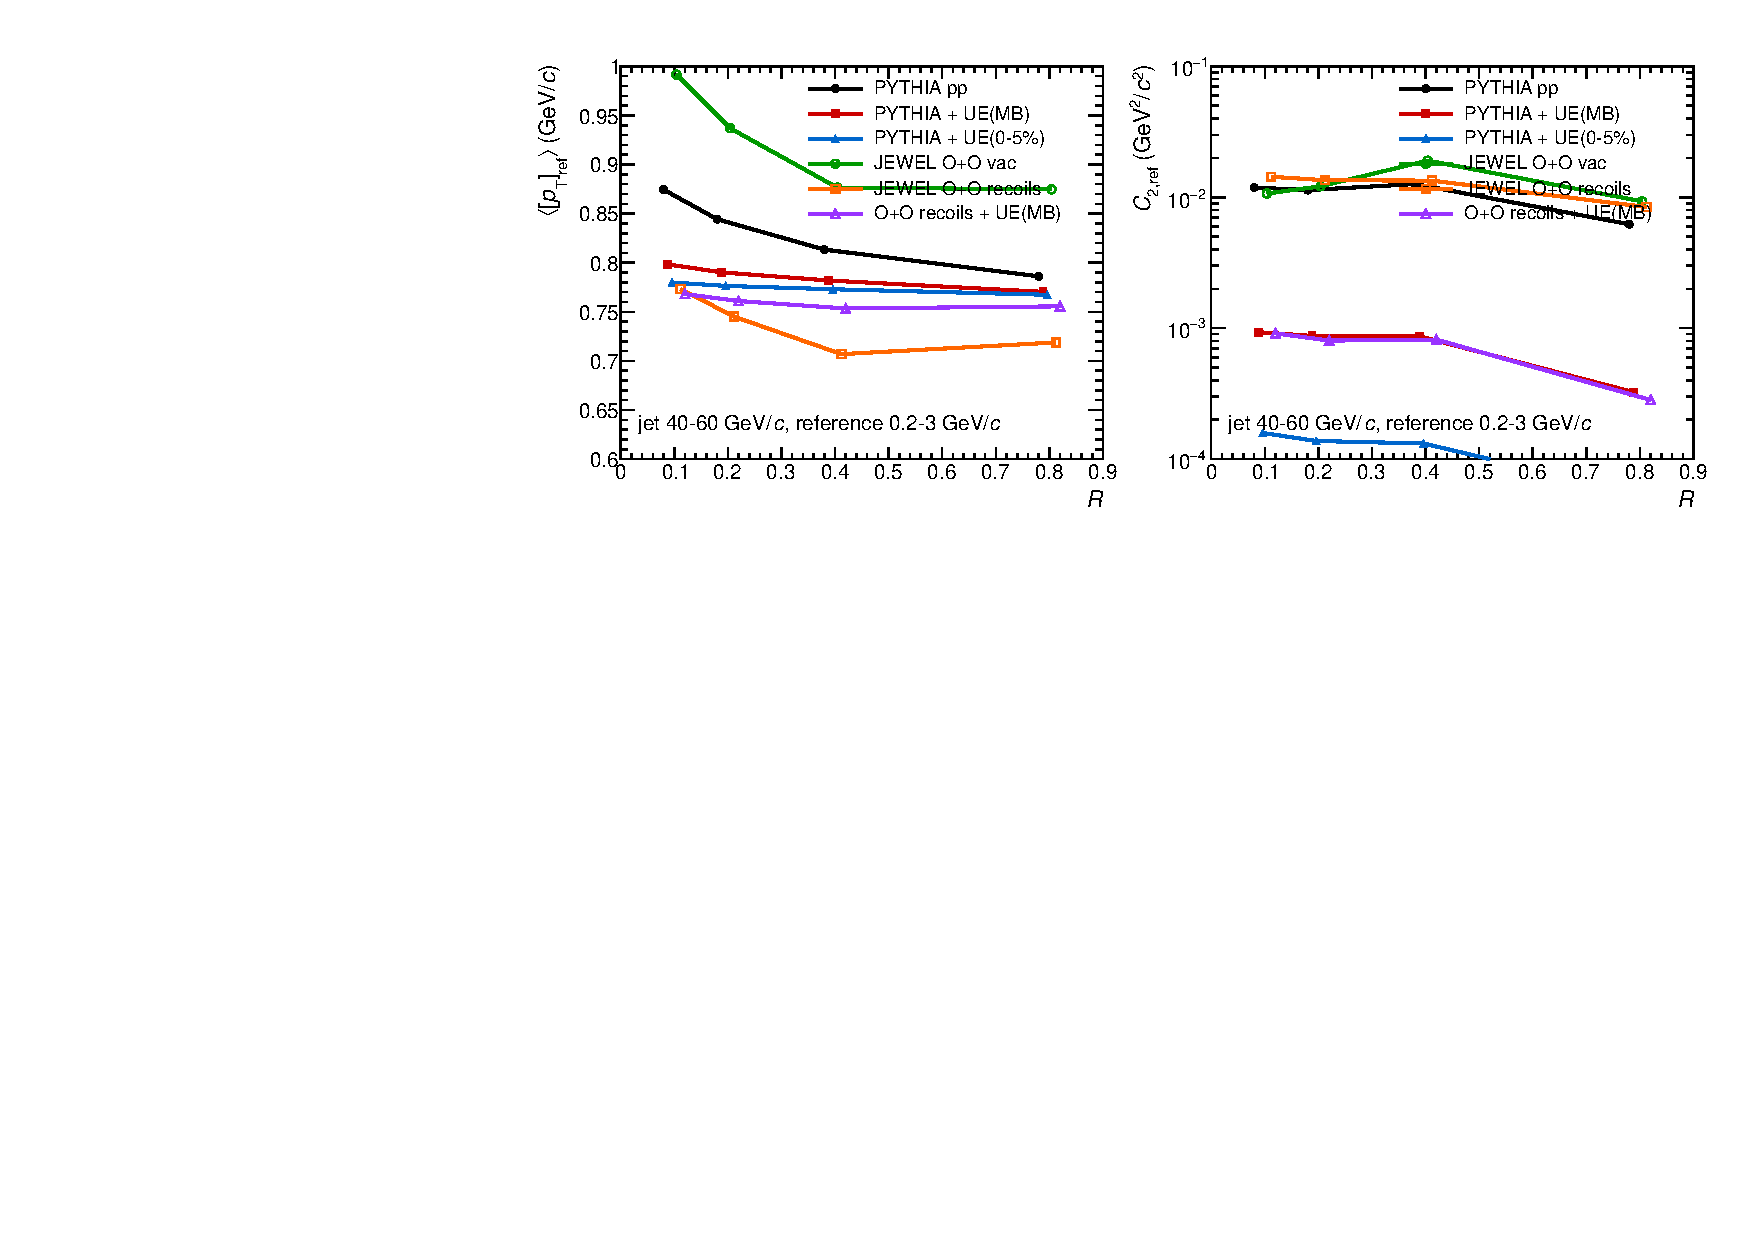
\includegraphics[width=0.98\textwidth]{figs/qa_reference.pdf}
\caption{Reference mean transverse momentum (left) and distinct-pair correlator (right) versus radius for the indicated generator and embedding configurations, with jet momentum $40$--$60$ GeV/$c$. The reference range is $0.2<\pT<3$ GeV/$c$. The $R=0.8$ point uses the wider tracking acceptance.}
\label{fig:qa_reference}
\end{figure*}

\begin{figure*}[tp]
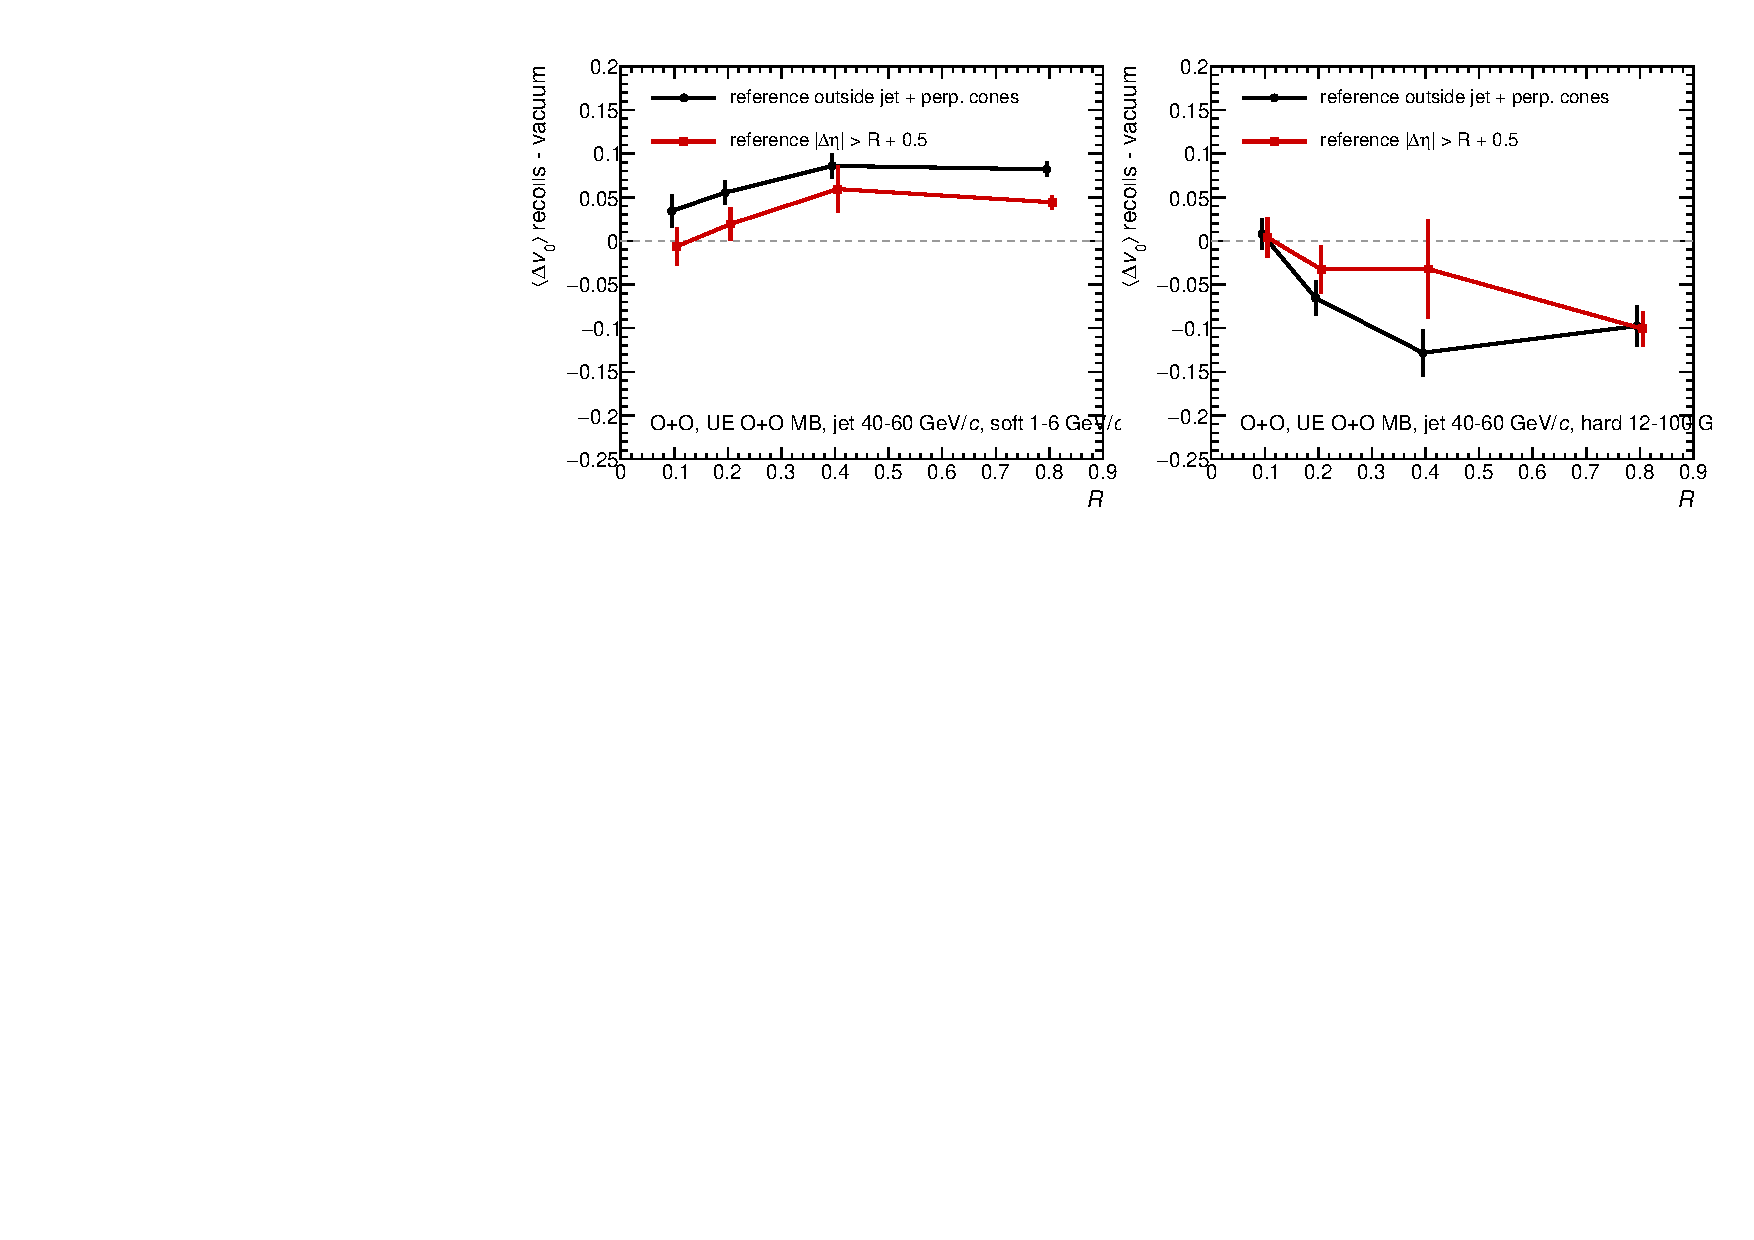
\includegraphics[width=0.98\textwidth]{figs/qa_refgap.pdf}
\caption{Medium-with-recoils minus vacuum at the same minimum-bias O+O embedding density for the nominal and pseudorapidity-separated reference. Left: soft probes. Right: hard probes. Jets have corrected momentum $40$--$60$ GeV/$c$. The reference change modifies both the covariance and its normalization.}
\label{fig:qa_gap}
\end{figure*}

\begin{figure*}[tp]
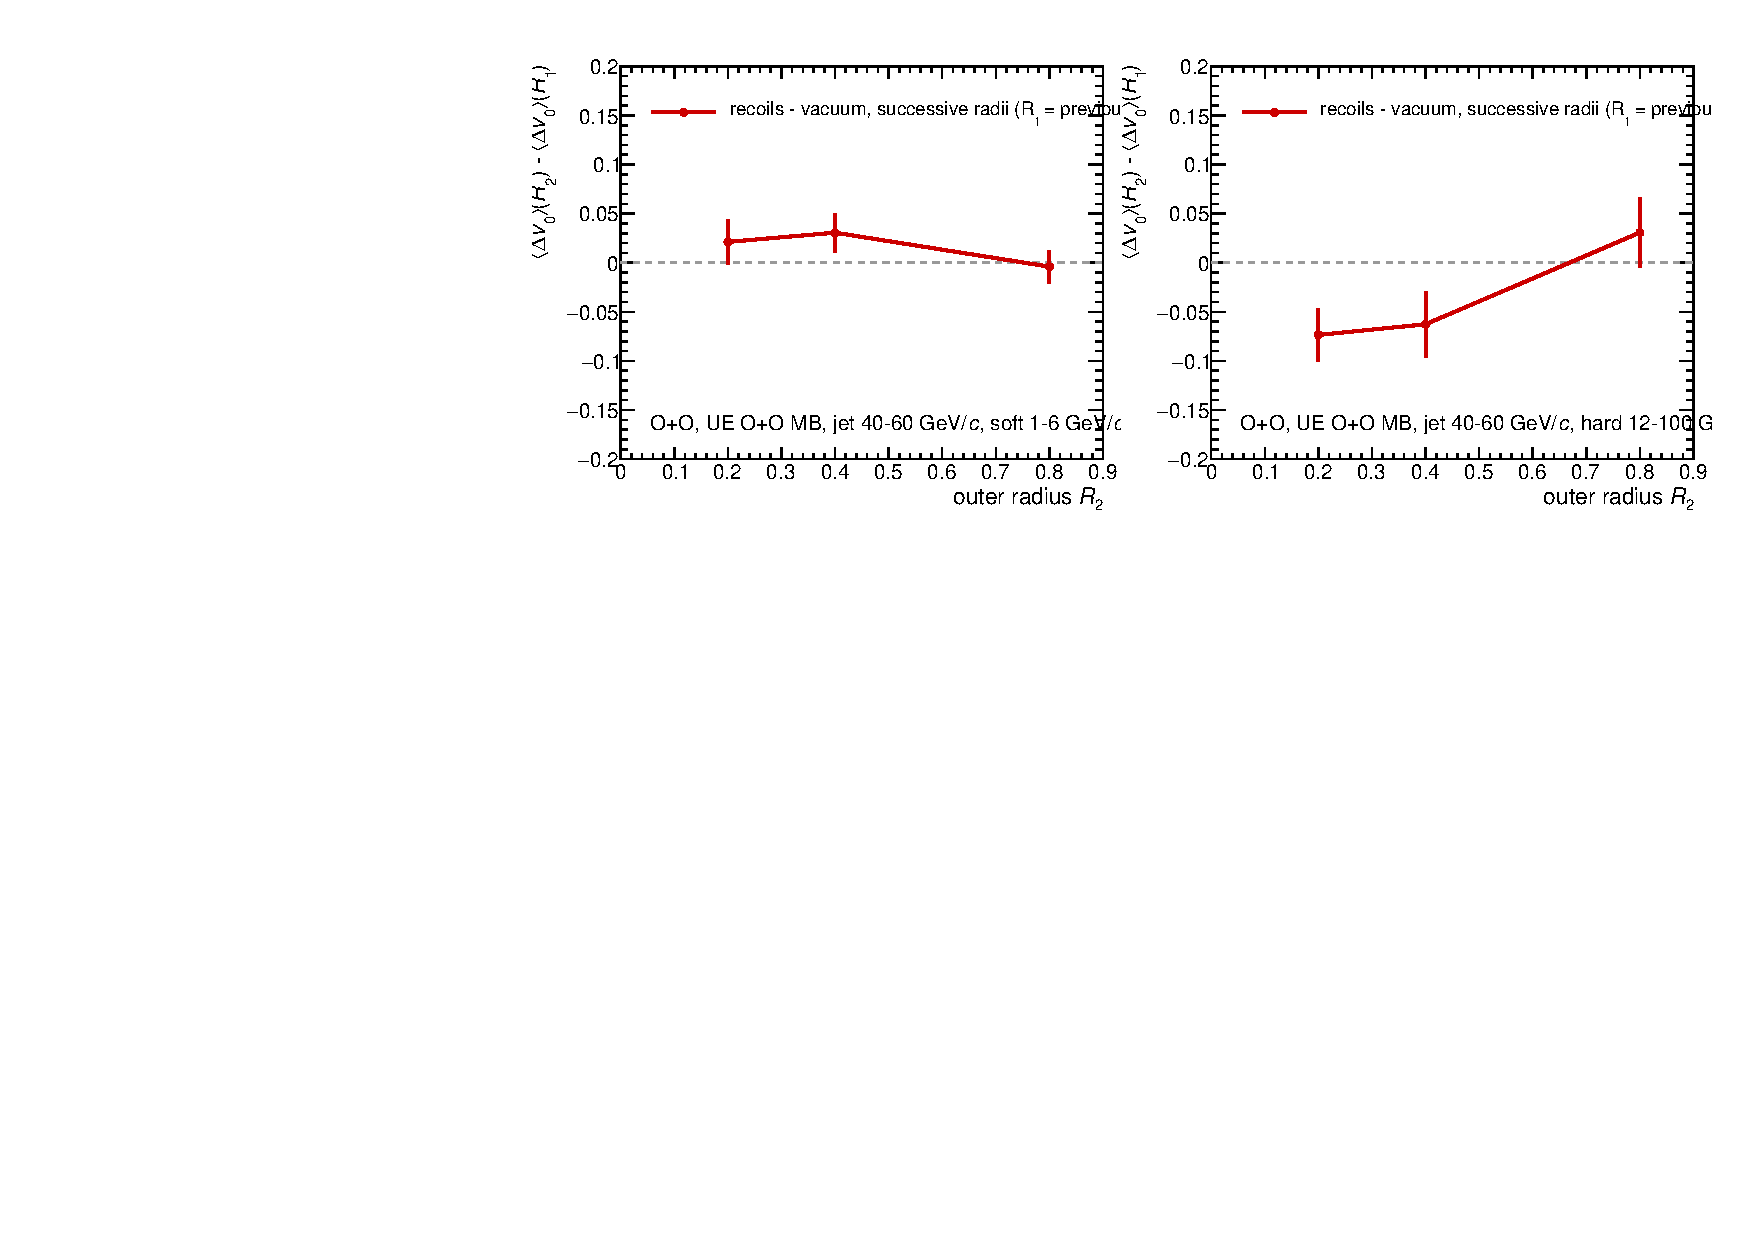
\includegraphics[width=0.98\textwidth]{figs/qa_annulus.pdf}
\caption{Difference of the recoil-retaining medium signal between successive radii. The horizontal coordinate is the larger radius; the smaller is the preceding value in $0.1,0.2,0.4,0.8$. Left: soft probes. Right: hard probes. Errors add the separate-radius uncertainties in quadrature without their covariance. These differences include changes of probe, reference, normalization, and selection; they are not annular yields.}
\label{fig:qa_radius}
\end{figure*}

\begin{figure*}[tp]
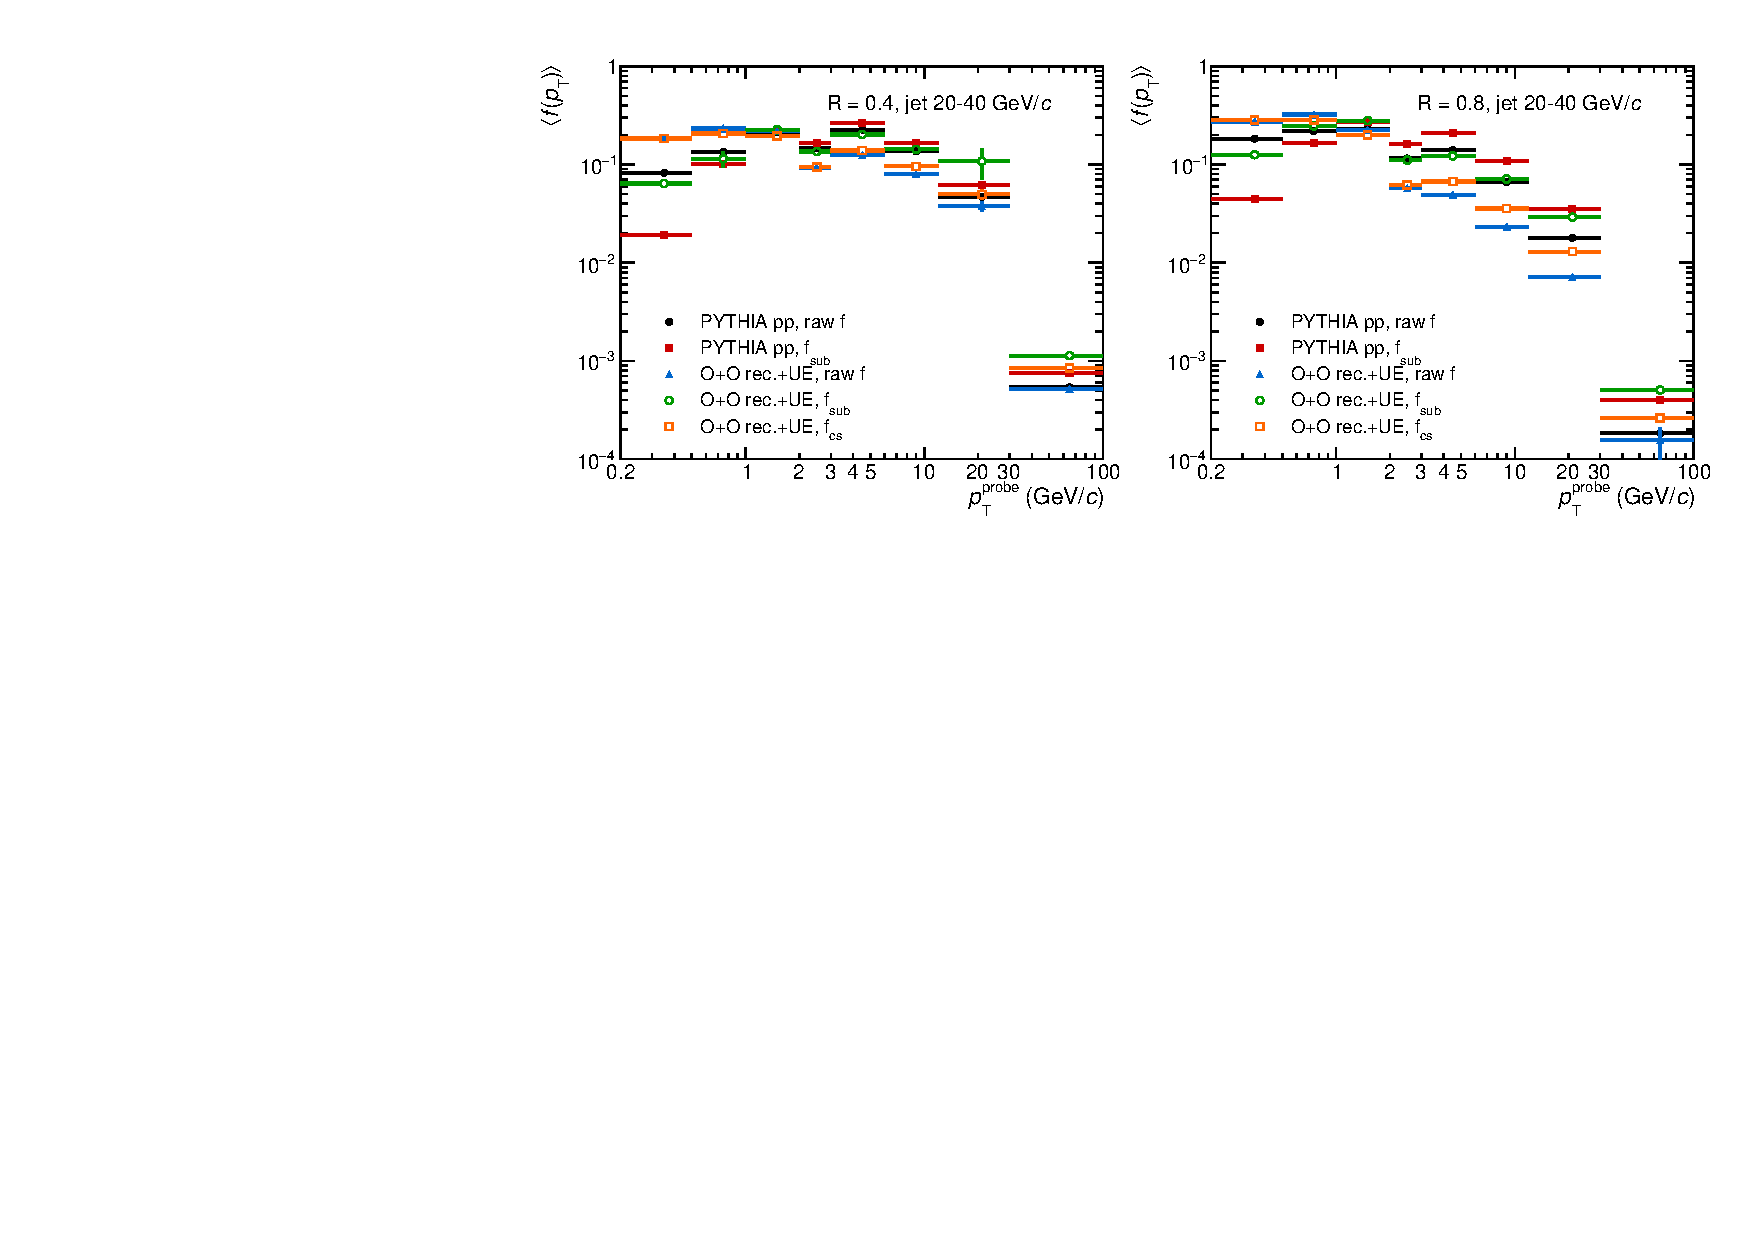
\includegraphics[width=0.98\textwidth]{figs/qa_fmean.pdf}
\caption{Mean normalized probe spectra for raw, perpendicular-cone-subtracted, and constituent-subtracted definitions in PYTHIA and in recoil-retaining JEWEL with embedding. Left and right panels show $R=0.4$ and $0.8$ for $20$--$40$ GeV/$c$ jets. The normalization conventions are those of Eqs.~\eqref{eq:f} and \eqref{eq:subtracted}.}
\label{fig:qa_fraction}
\end{figure*}

\begin{figure*}[tp]
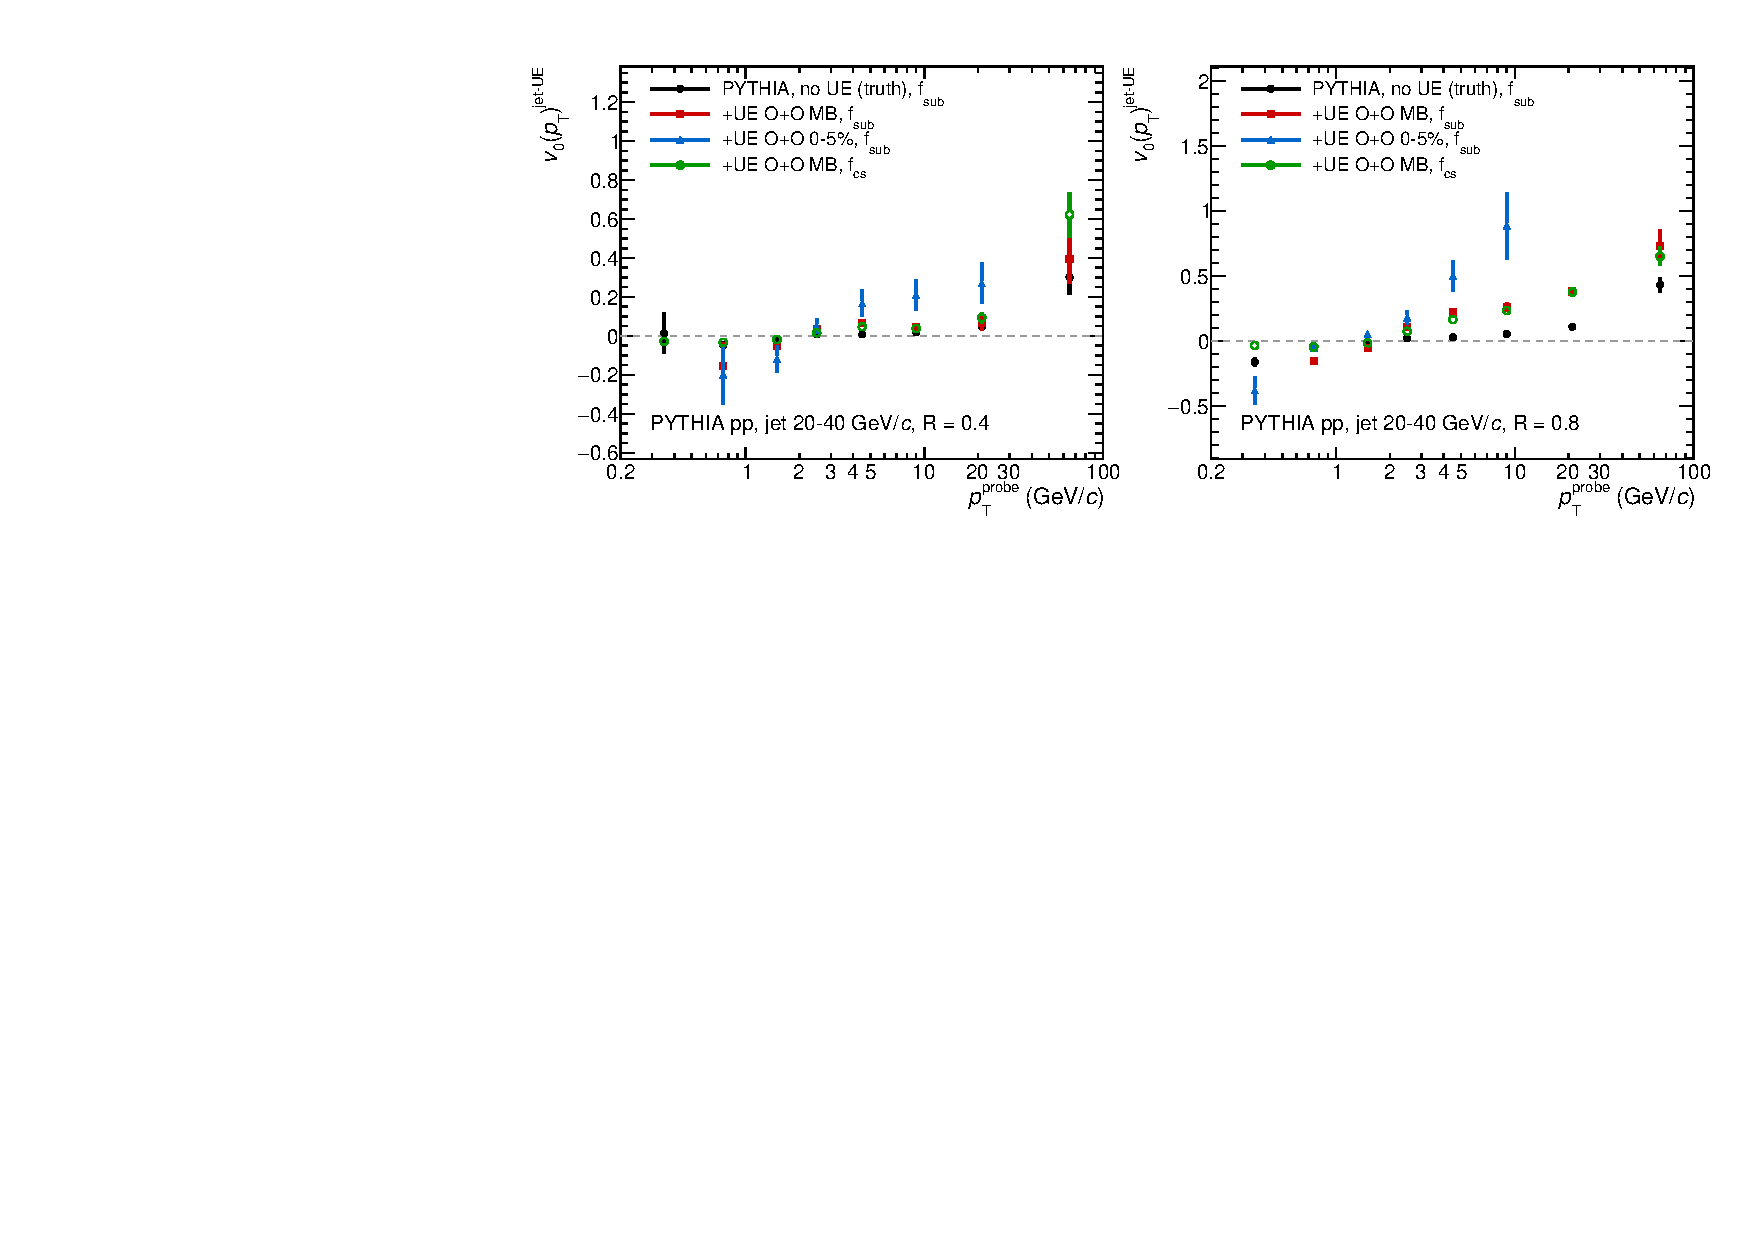
\includegraphics[width=0.98\textwidth]{figs/qa_closure.pdf}
\caption{Vacuum embedding check in PYTHIA for $20$--$40$ GeV/$c$ jets: the unembedded result and the results after embedding at the minimum-bias and central O+O background densities. Perpendicular-cone and constituent subtraction are compared. A difference from the unembedded result includes changes of selection and reference composition and contributes to the background baseline.}
\label{fig:qa_closure}
\end{figure*}

\begin{figure*}[tp]
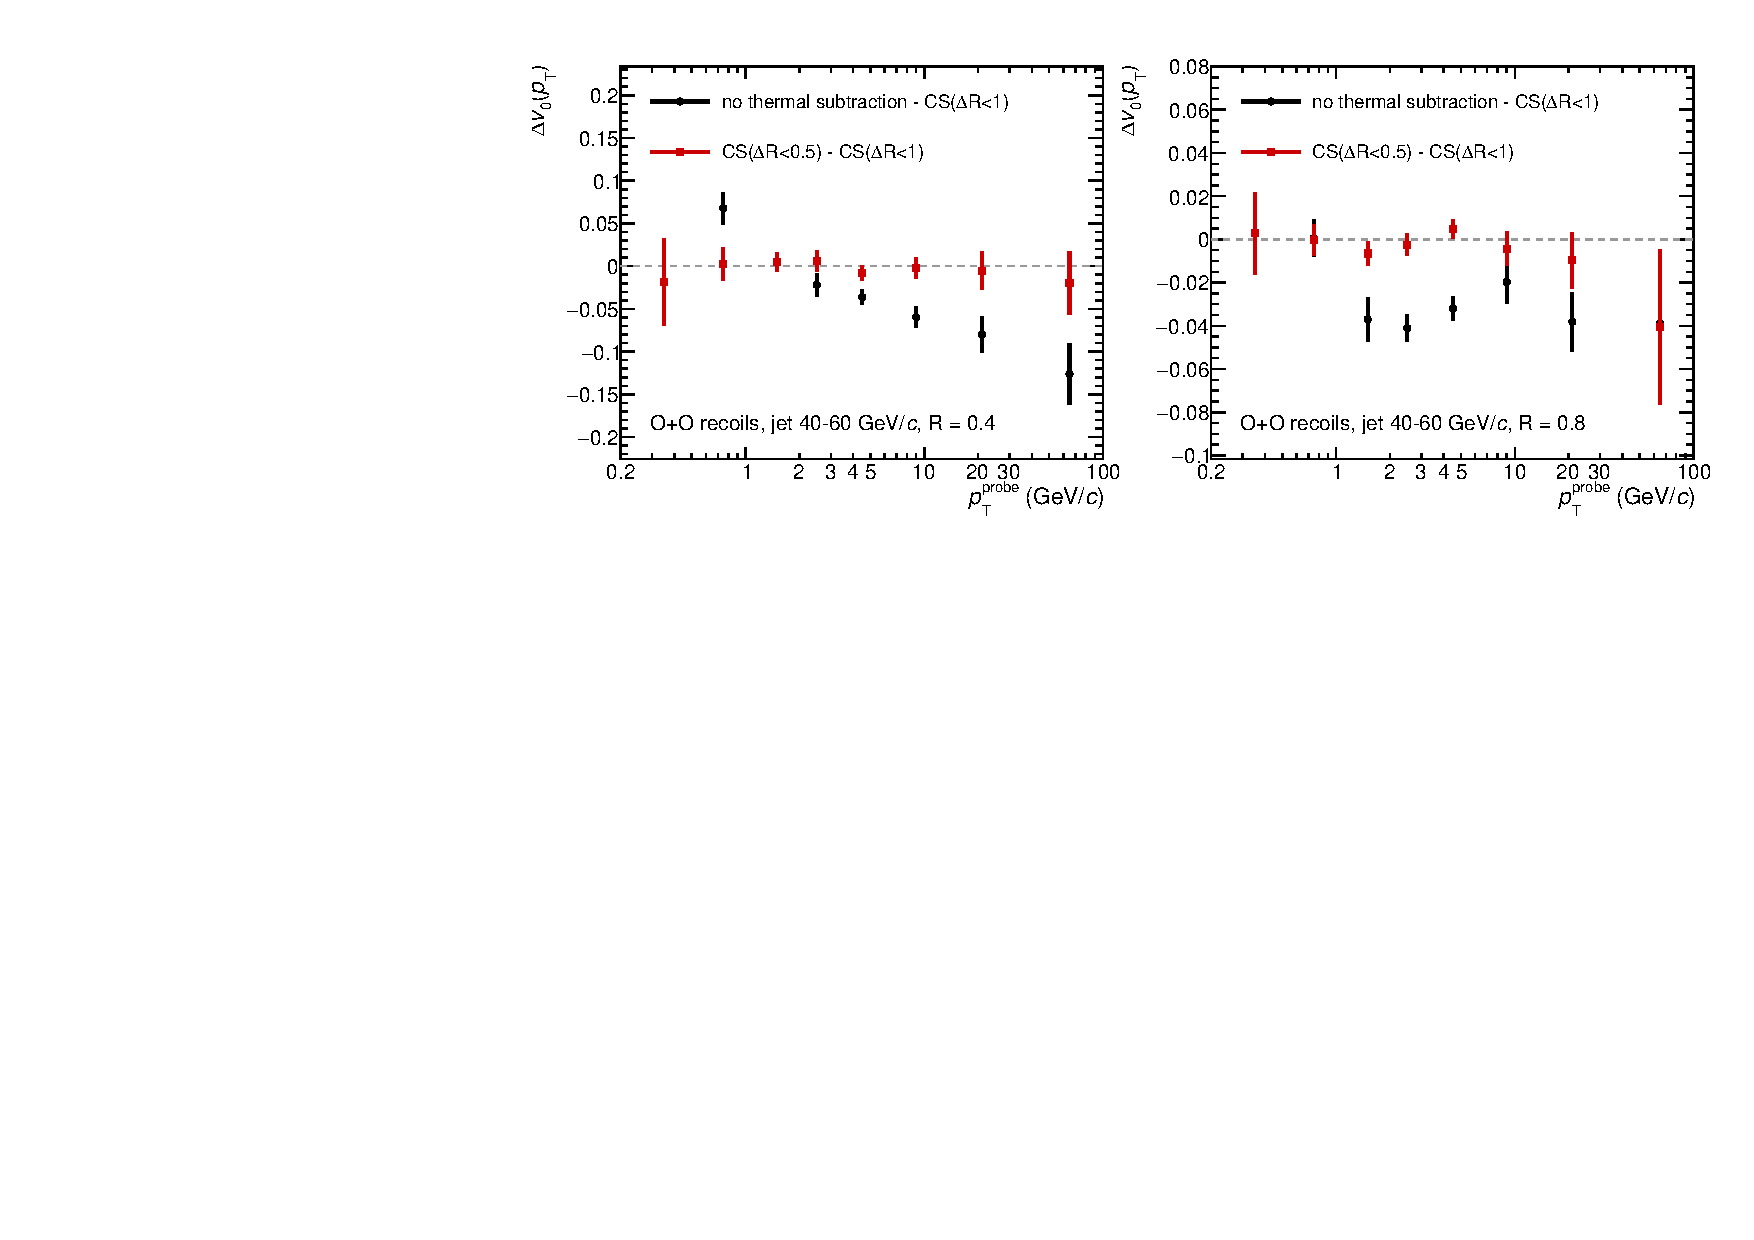
\includegraphics[width=0.98\textwidth]{figs/qa_recoilsub.pdf}
\caption{Change of the recoil-retaining result relative to nominal thermal-momentum subtraction with maximum distance $1.0$. The alternatives omit the subtraction or use maximum distance $0.5$. Panels show $R=0.4$ and $0.8$ for $40$--$60$ GeV/$c$ jets. This concerns pre-scattering thermal recoil momenta, not subtraction of the independently embedded background.}
\label{fig:qa_recoil}
\end{figure*}


\end{document}
